\documentclass{sigchi}

% Use this section to set the ACM copyright statement (e.g. for
% preprints).  Consult the conference website for the camera-ready
% copyright statement.

% Copyright
\CopyrightYear{2016}
%\setcopyright{acmcopyright}
\setcopyright{acmlicensed}
%\setcopyright{rightsretained}
%\setcopyright{usgov}
%\setcopyright{usgovmixed}
%\setcopyright{cagov}
%\setcopyright{cagovmixed}
% DOI
\doi{http://dx.doi.org/10.475/123_4}
% ISBN
\isbn{123-4567-24-567/08/06}
%Conference
\conferenceinfo{CHI'16,}{May 07--12, 2016, San Jose, CA, USA}
%Price
\acmPrice{\$15.00}

% Use this command to override the default ACM copyright statement
% (e.g. for preprints).  Consult the conference website for the
% camera-ready copyright statement.

%% HOW TO OVERRIDE THE DEFAULT COPYRIGHT STRIP --
%% Please note you need to make sure the copy for your specific
%% license is used here!
% \toappear{
% Permission to make digital or hard copies of all or part of this work
% for personal or classroom use is granted without fee provided that
% copies are not made or distributed for profit or commercial advantage
% and that copies bear this notice and the full citation on the first
% page. Copyrights for components of this work owned by others than ACM
% must be honored. Abstracting with credit is permitted. To copy
% otherwise, or republish, to post on servers or to redistribute to
% lists, requires prior specific permission and/or a fee. Request
% permissions from \href{mailto:Permissions@acm.org}{Permissions@acm.org}. \\
% \emph{CHI '16},  May 07--12, 2016, San Jose, CA, USA \\
% ACM xxx-x-xxxx-xxxx-x/xx/xx\ldots \$15.00 \\
% DOI: \url{http://dx.doi.org/xx.xxxx/xxxxxxx.xxxxxxx}
% }

% Arabic page numbers for submission.  Remove this line to eliminate
% page numbers for the camera ready copy
% \pagenumbering{arabic}

% Load basic packages
\usepackage{balance}       % to better equalize the last page
\usepackage{graphics}      % for EPS, load graphicx instead
\usepackage[T1]{fontenc}   % for umlauts and other diaeresis
\usepackage{txfonts}
\usepackage{mathptmx}
\usepackage[pdflang={en-US},pdftex]{hyperref}
\usepackage{color}
\usepackage{booktabs}
\usepackage{textcomp}
% Some optional stuff you might like/need.
\usepackage{microtype}        % Improved Tracking and Kerning
% \usepackage[all]{hypcap}    % Fixes bug in hyperref caption linking
\usepackage{ccicons}          % Cite your images correctly!
% \usepackage[utf8]{inputenc} % for a UTF8 editor only

% If you want to use todo notes, marginpars etc. during creation of
% your draft document, you have to enable the "chi_draft" option for
% the document class. To do this, change the very first line to:
% "\documentclass[chi_draft]{sigchi}". You can then place todo notes
% by using the "\todo{...}"  command. Make sure to disable the draft
% option again before submitting your final document.
\usepackage{todonotes}
\usepackage{enumitem}
% Paper metadata (use plain text, for PDF inclusion and later
% re-using, if desired).  Use \emtpyauthor when submitting for review
% so you remain anonymous.
% \def\plaintitle{Do You Like Comics? Using Algorithmically Synthesized Comic-Style Messages to Persuade Behavioral Change
% }
% \def\plaintitle{It's comical: dressing facts with comics}
% \def\plaintitle{It's comical: persuasive facts with comics}
\def\plaintitle{It's Comical: When Facts in Comic Form Persuade}

\def\plainauthor{First Author, Second Author, Third Author,
Fourth Author, Fifth Author, Sixth Author}
\def\emptyauthor{}
\def\plainkeywords{Authors' choice; of terms; separated; by
semicolons; include commas, within terms only; required.}
\def\plaingeneralterms{Documentation, Standardization}

% llt: Define a global style for URLs, rather that the default one
\makeatletter
\def\url@leostyle{%
 \@ifundefined{selectfont}{
  \def\UrlFont{\sf}
  }{
  \def\UrlFont{\small\bf\ttfamily}
}}
\makeatother
\urlstyle{leo}

% To make various LaTeX processors do the right thing with page size.
\def\pprw{8.5in}
\def\pprh{11in}
\special{papersize=\pprw,\pprh}
\setlength{\paperwidth}{\pprw}
\setlength{\paperheight}{\pprh}
\setlength{\pdfpagewidth}{\pprw}
\setlength{\pdfpageheight}{\pprh}

% Make sure hyperref comes last of your loaded packages, to give it a
% fighting chance of not being over-written, since its job is to
% redefine many LaTeX commands.
\definecolor{linkColor}{RGB}{6,125,233}
\hypersetup{%
 pdftitle={\plaintitle},
 % Use \plainauthor for final version.
 %  pdfauthor={\plainauthor},
 pdfauthor={\emptyauthor},
 pdfkeywords={\plainkeywords},
 pdfdisplaydoctitle=true, % For Accessibility
 bookmarksnumbered,
 pdfstartview={FitH},
 colorlinks,
 citecolor=black,
 filecolor=black,
 linkcolor=black,
 urlcolor=linkColor,
 breaklinks=true,
 hypertexnames=false
}

% create a shortcut to typeset table headings
% \newcommand\tabhead[1]{\small\textbf{#1}}

% End of preamble. Here it comes the document.
\begin{document}

\title{\plaintitle}

\numberofauthors{3}
\author{%
 \alignauthor{Leave Authors Anonymous\\
  \affaddr{for Submission}\\
  \affaddr{City, Country}\\
  \email{e-mail address}}\\
 \alignauthor{Leave Authors Anonymous\\
  \affaddr{for Submission}\\
  \affaddr{City, Country}\\
  \email{e-mail address}}\\
 \alignauthor{Leave Authors Anonymous\\
  \affaddr{for Submission}\\
  \affaddr{City, Country}\\
  \email{e-mail address}}\\
}

\maketitle

% \begin{abstract}
%    %!TEX root = proceedings.tex

Interest in the role of technology in behavior
change has been growing over the recent years.
Social network users are exposed to massive
information while they are reading their
newsfeed and interacting with their friends.
Attracting people's limited attention has been
a critical question in online persuasive technology.
Previous works have demonstrated that messages are
more attractive in a graphical form than plain text,
however, whether the comic messages can persuade the
reader and engage behavior change remains unknown.
This paper presents a research on the persuasiveness of
comic style messages. We showed that people perceive a message as more
persuasive when it is in a comic form than in plain text.
Then, we further investigated how different elements in
a comic message could influence the persuasive power of the message.

% \end{abstract}
\section{ABSTRACT}
%!TEX root = proceedings.tex

Interest in the role of technology in behavior
change has been growing over the recent years.
Social network users are exposed to massive
information while they are reading their
newsfeed and interacting with their friends.
Attracting people's limited attention has been
a critical question in online persuasive technology.
Previous works have demonstrated that messages are
more attractive in a graphical form than plain text,
however, whether the comic messages can persuade the
reader and engage behavior change remains unknown.
This paper presents a research on the persuasiveness of
comic style messages. We showed that people perceive a message as more
persuasive when it is in a comic form than in plain text.
Then, we further investigated how different elements in
a comic message could influence the persuasive power of the message.

% \begin{method}
%    %!TEX root = cscw2018-comic.tex

\section{Study on Preference: Method}
\label{sec:preference}
% \subsection{Method}
% \label{sec:Method}

In this section, we discuss our methodology for evaluating the preference of the message shown in the abstract comic form over the plain text message. First we discuss the messages used with positive and negative framing. Then, we show how to synthesize the abstract comic messages. Then we discuss our HIT design on the Mechanical Turk.

% how we instantiated the study on Amazon Mechanical Turk, followed by a discussion of how we evolved our experiment design based on Turker feedback. We conclude this section with a discussion of how we identified potential subjects on Amazon Mechanical Turk.

\subsection{Composing Persuasive Messages in Plain Text}
We use simple text messages with a goal to persuade subjects to engage more physical activity. We chose this topic as the health is a topic to which our study participants could relate. We kept a single topic to avoid any any experimental confounds due to different topics.

% Aligned with the idea of memorability, the main theme of all persuasive messages and simple, persuading the target persuadee to engage more physical activity. The main reasons to choose this topics are 1) As a basic daily activity everyone has the need to exercise. 2) People can easily understand the message and relate to themselves. 3) Engaging more exercise is mostly based on audience own willingness instead of any other subjective resources.

We constructed messages based on the idea of social proof~\cite{goldstein2008room}, where the messages emphasized the relationship between the subject and her group of friends. We created two sets of messages that either framed from a positive standpoint or a negative standpoint \cite{tversky1981framing}.

We used the following positive and negatively framed messages in our study.
\textit{Positive framed persuasive messages:}
\begin{enumerate}
	\item In the past week, you spent more time at the gym than did 65\% of your friends
	\item Congrats! You have reached your goal of exercising three times a week.
	\item Over the past month, you exercised more than did 90\% of your friends.
	\item Your exercise activity is in the top 20\% of all your friends.
	\item Over the past three weeks, you went to the gym more often than 60\% of your friends did.
\end{enumerate}\par
\textit{Negative framed persuasive messages:}
\begin{enumerate}
	\item	In the past week, you spent less time at the gym than did 65\% of your friends
	\item  Oh! You did not reach your goal of exercising three times a week.
	\item	Over the past month, you exercised less than did 90\% of your friends.
	\item	Your exercise activity is in the bottom 20\% of all your friends.
	\item	Over the past three weeks, you went to the gym less often than 60\% of your friends did.
\end{enumerate}

\subsection{Generating Comics}
In this study, we adapted an open source comic generator~\cite{cmx.io} to generate abstract comic messages. The generator impersonates the style found on 'XKCD'~\cite{munroe2009xkcd} comic. Our focus is not the XKCD style, but the fact that the comic form generated by~~\cite{cmx.io} is abstract. The message we generate includes two characters in a conversation and the scenario is `One day, your friend has something to tell you.'

\begin{figure}[t]
	\centering
	\begin{tabular}{cc}
		\subfloat[Gestures for positive framed messages]{\label{figur:1a}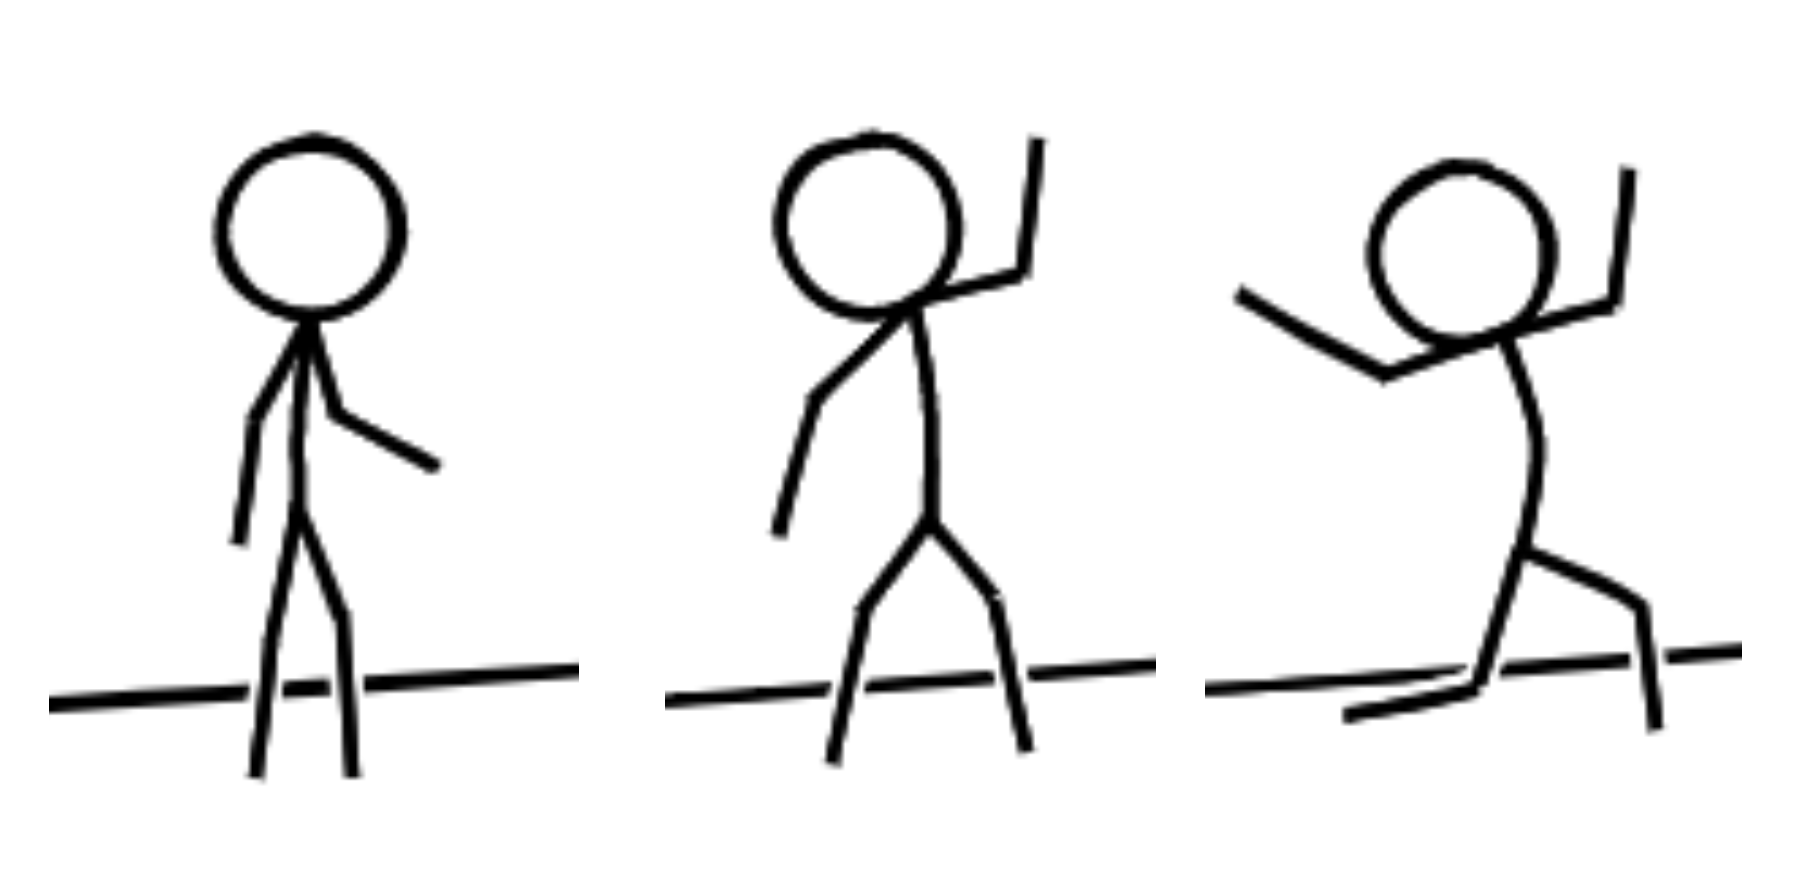
\includegraphics[width = 0.4\columnwidth]{figures/pos_figures}} &
		\subfloat[Gesture for negative framed messages ]{\label{figur:1b}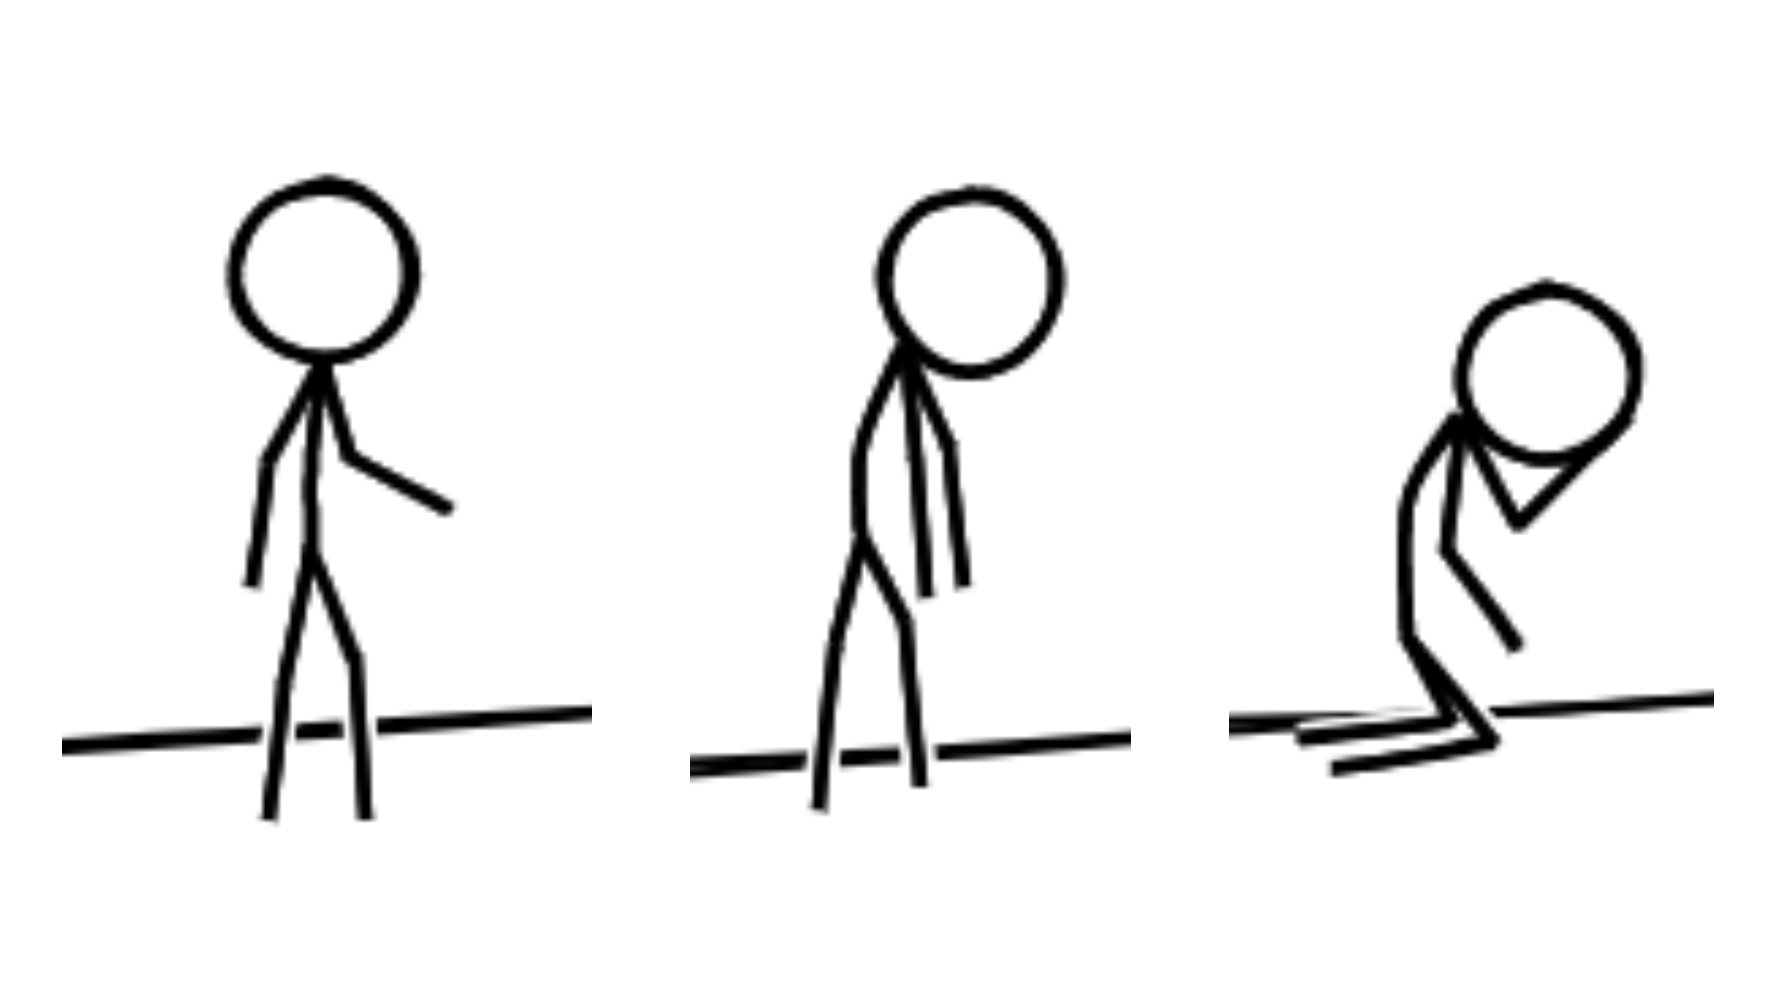
\includegraphics[width = 0.4 \columnwidth]{figures/neg_figures}}\\
	\end{tabular}
	\caption{Different character gestures to communicate various levels of emotional intensity. The left figure shows gestures used in positive framed messages from neutral to the happiest. The right figure shows gesture used in negative framed messages from neutral to the most frustrated. }
	\label{figur:figures}
\end{figure}

% \begin{figure}[t]
% 	\centering
% 	\begin{tabular}{ccc}
% 		\subfloat[Close Friends]{\label{figur:3a}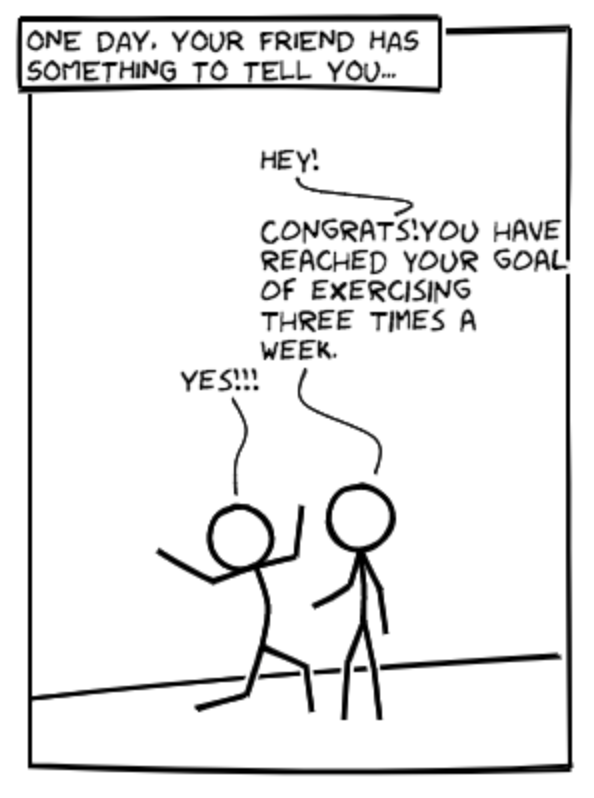
\includegraphics[width = 0.27\columnwidth]{figures/d0}} &
% 		\subfloat[Friends]{\label{figur:3b}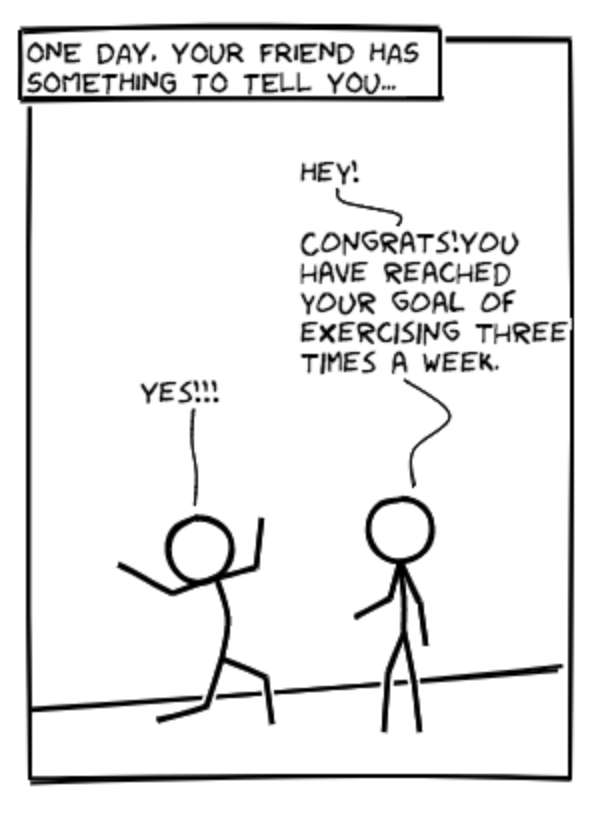
\includegraphics[width = 0.27 \columnwidth]{figures/d1}}      &
% 		\subfloat[Acquaintance]{\label{figur:3c}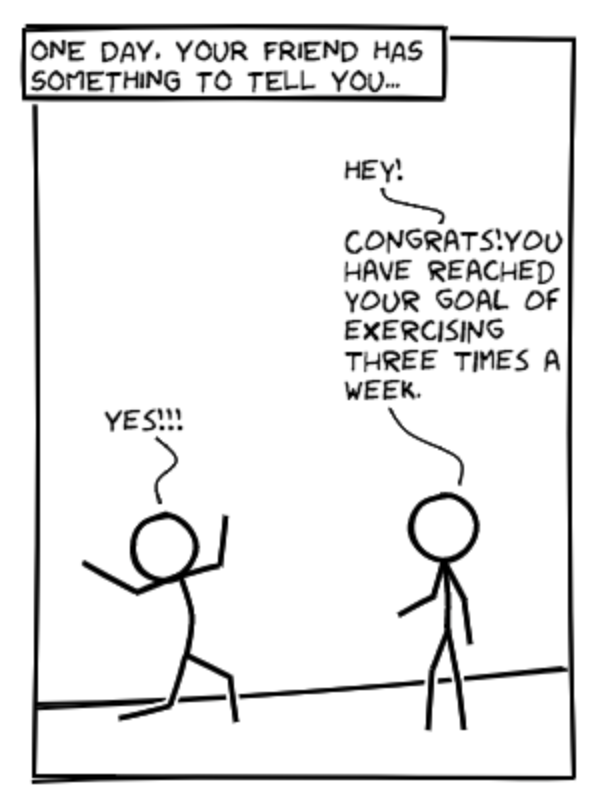
\includegraphics[width = 0.27 \columnwidth]{figures/d2}}\\
% 	\end{tabular}
% 	\caption{Different distance to communicate various levels of relationship closeness}
% 	\label{figur:distance}
% \end{figure}

To make a fair comparison between plain text representation and the comic form, the content of text bubble is the same in both conditions. We discuss generation of elements of gesture, distance between characters and shading below.

\begin{description}
	\item[Gesture]: We created the gesture library with two main categories: positive and negative corresponding to how the original message is framed, each with three levels of emotional intensity see Figure~\ref{figur:figures}.
	\item[Inter-character distance]: For the distance between two characters, we have three levels of variance from close to medium separation to large separation. The three levels of distance represents the relationship between to characters as close friends, friends, and acquaintances.
	\item[Shading]: For the background shading, we have three-levels , white, grey, and dark grey. Each color represents a level of emotional intensity correspondingly, white as ~\cite{scott1993understanding}.
\end{description}


% \begin{figure}[]
% 	\centering
% 	\begin{tabular}{ccc}
% 		\subfloat[Lowest]{\label{figur:4a}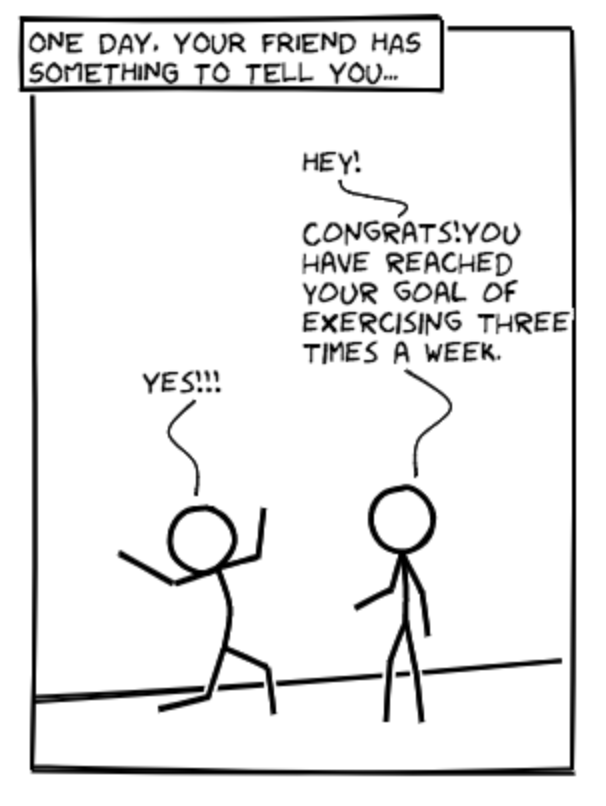
\includegraphics[width = 0.27\columnwidth]{figures/s0}}    &
% 		\subfloat[Moderate]{\label{figur:4b}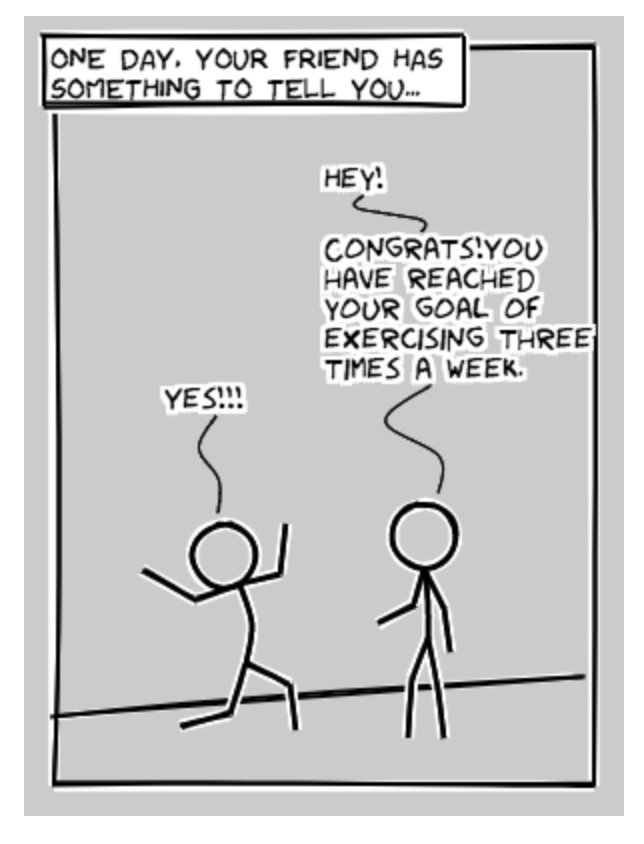
\includegraphics[width = 0.27 \columnwidth]{figures/s1}} &
% 		\subfloat[Intense]{\label{figur:4c}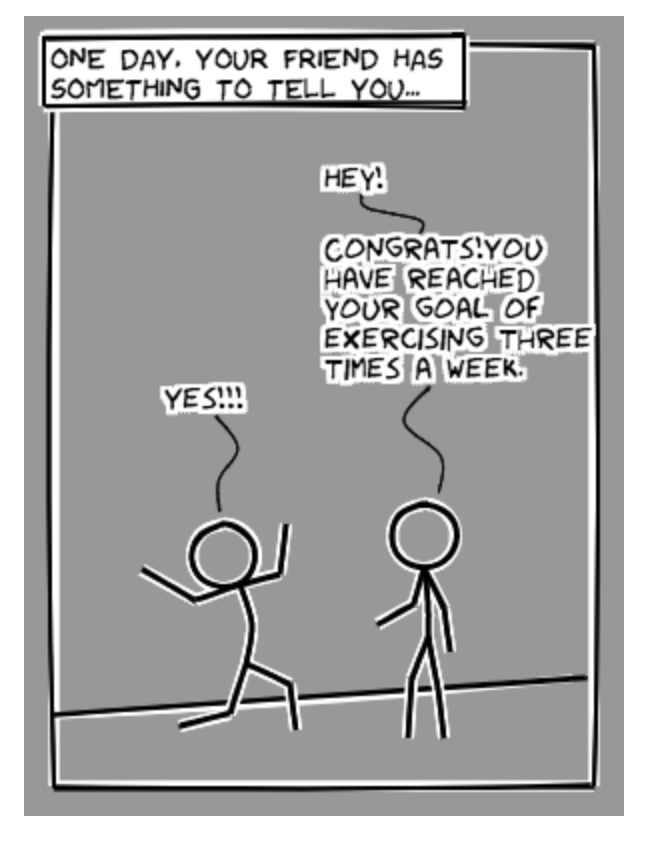
\includegraphics[width = 0.27 \columnwidth]{figures/s2}}\\
% 	\end{tabular}
% 	\caption{Different background to communicate various levels of emotional intensity}
% 	\label{figur:shading}
% \end{figure}

In total, for each message we have a total of $3 \times 3 \times 3 \times 2 =54$ variations in terms of character gesture, inter-character, background shading, and message framing. In this study, we created 270 comic form messages corresponding to 5 plain text messages.

Since the prior work~\cite{goldstein2008room,schultz2007constructive} suggests a robust effect of the social proof, instead of using it as part of an experimental condition, we will have two characters in the comic, shown as friends or the experimenter, whose inter-character distance we manipulate. Second, we will incorporate framing in the text bubbles accompanying the comic.

\subsection{Study Design}
To answer our research questions, we designed and after IRB approval, conducted a between-subject online study on Amazon Mechanical Turk.

\textit{Experiment Procedure.} Once participant consented to join our study, they were randomly assigned to two conditions 1) Positive message condition where all persuasive messages are framed in a positive way and 2) Negative condition where all persuasive messages are framed in a negative way. In both conditions, participants will see a total of five persuasive messages in both plain-text representation and comic representation shown side by side. Then, the participant rates which representation of the message is perceived as more persuasive on a 7-item Likert scale.

\textit{Display Order.} To mitigate any potential bias toward the display order of the plain-text representation and comic representation we randomize the display order. Both plain-text representation and comic-style representation have equal chance to show on the left side.

\textit{Attention Checker.} To control the data quality, we embedded two attention checkers in the study. The first one appears after the third comparison and the second one shows up after the last comparison. Both attention checkers asked subjects to choose a comic that matches a simple description, e.g. ``Which of the following comics has two characters?''

\textit{Rating Scale Design.} The 7-item Likert scale ranges from -3 (left) to 3 (right) where 0 means neutral. The direction of the scale flips corresponding to the position of the comic and plain text.
%see the right part of Figure~\ref{fig:change}.

\textit{A Pilot Study.} Before the experiment, we first conducted a pilot study with 10 participants and collect their opinions about the study process and design. Based on the feedback from our pilot test, we iterated our study design. In the final design, we fixed the order of the rating scale. However, since the order is fixed, potential demand characteristics may be introduced by the scale direction~\cite{orne1962social}. To minimize potential bias we added another layer of randomness in our final design. The direction of the scale no longer changes respect to the position of the messages within subjects, but the direction of the scale is randomly assigned between subjects. Also, we replaced the numbers on the scale by text as neutral, slightly persuasive, text/comics is more persuasive and strongly persuasive. Finally, we adjusted the size of the comic and text to make sure both of them have similar readability.
%
% The left side of Figure~\ref{fig:change} shows the final design. Another round of pilot study with another 10 participants showed the newer design successfully addressed the problems in the old design and we encountered no new problems.

% \begin{figure}
%  \centering
%  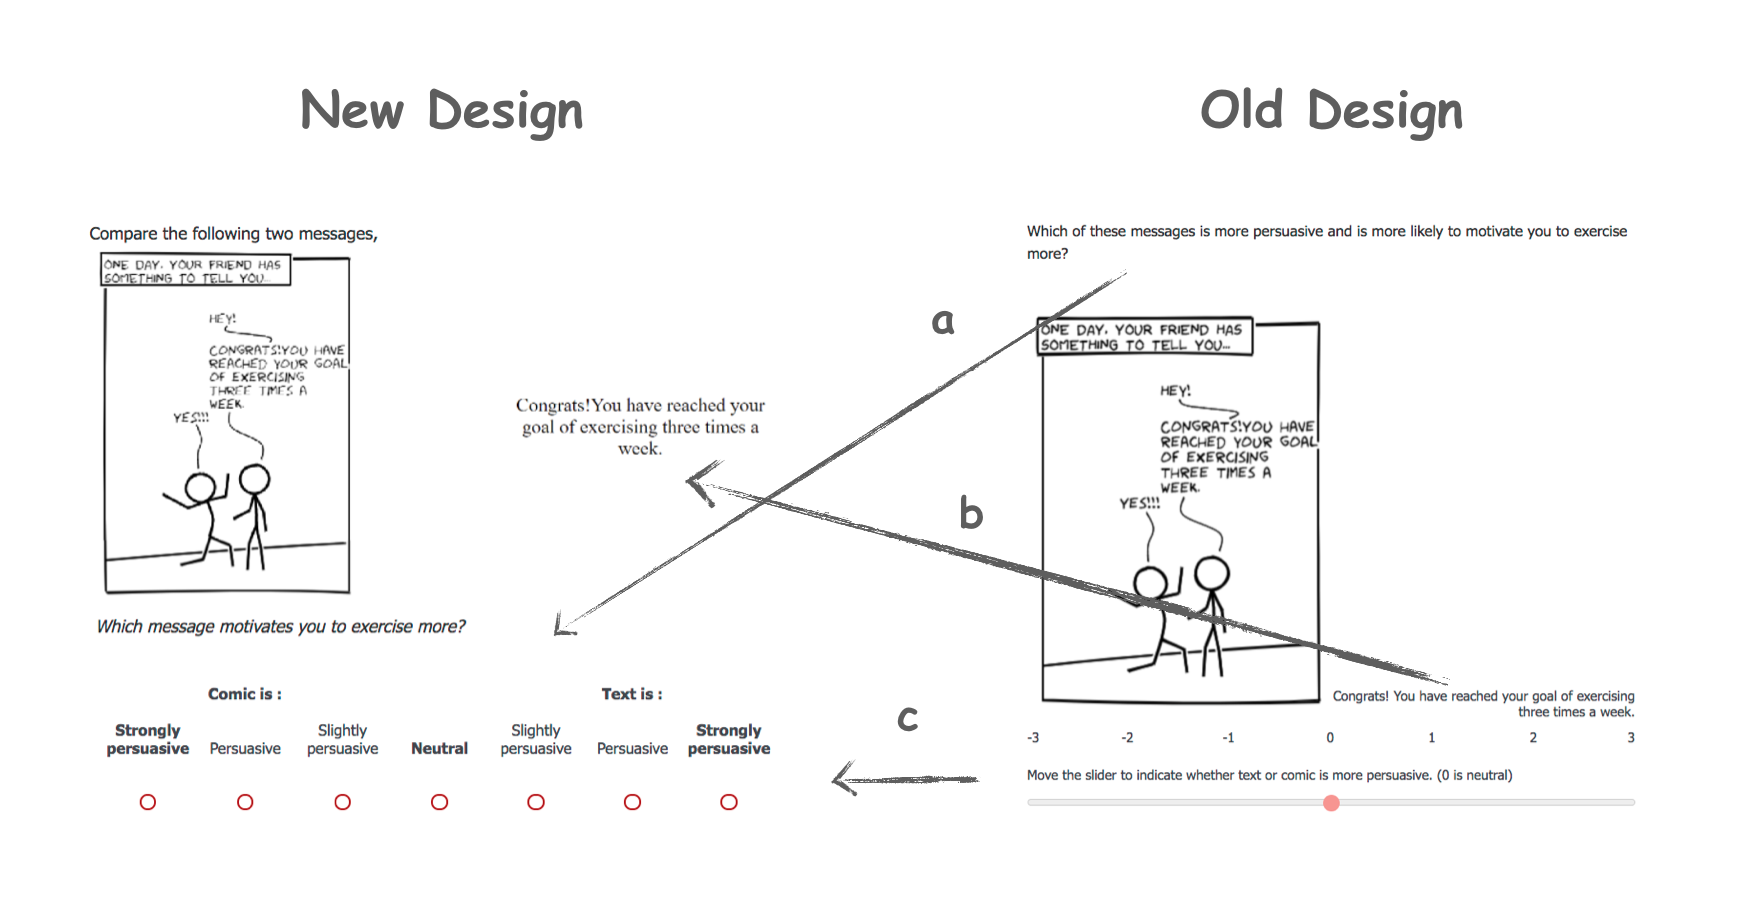
\includegraphics[width=0.95\columnwidth]{figures/change}
%  \caption{Design of the task before and after the pilot study. A. Change the position of the question to makes the question more clear. B. Adjust the position and the size of the text message to improve readability. C. Improve the rating scale to make it easy to interpreted.}
%  \label{fig:change}
% \end{figure}


\subsubsection{Participants}
We published our HITs on the Amazon Mechanical Turk titled with ``A short survey about your exercise motivation.'' The price tag for each HIT was \$8/hr, and the workers would get these rewards regardless of their performance. The threshold for participant to join our study was a 95\% Approval Rate. On the HIT page, participants would see a link to our experiment site. Workers who repeat the task will be rejected as we instructed in the task description.

% \end{method}

\category{H.5.m.}{Information Interfaces and Presentation
 (e.g. HCI)}{Miscellaneous} \category{See
 \url{http://acm.org/about/class/1998/} for the full list of ACM
 classifiers. This section is required.}{}{}

\keywords{\plainkeywords}
\newpage
\section{Introduction}
%!TEX root = cscw2019-comic.tex

% what is the problem?

% why is it important? what is the impact? what motivates?

% who else has done it?
% what did you do?

\section{introduction}
\label{sec:introduction}

\begin{wrapfigure}{R}{0.23\textwidth}
    \centering
    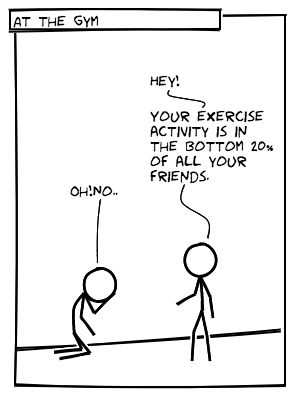
\includegraphics[width=0.21\textwidth]{figures/intro_new.png}
  \vspace{-10pt}
  \caption{The use of an abstract comic form.} \label{fig:intro}
  \vspace{-10pt}
\end{wrapfigure}

%From engaging collective action participation to individual health tracking, persuasion play an important role in nudging people to take the action.
Are text messages (e.g. ``"Would you like to donate to support the Organization for Autism Research?"'') more persuasive when expressed in comic\footnote{We use ``comic form'' as opposed to the more formal ``graphic form'' to avoid any confusion with other visual representations of data, including charts and diagrams.} form? Embellishing a text message using a comic form appears to be a ``Supposedly Irrelevant Factor''~\cite{Thaler2015}, that ought to make no difference to a decision maker since the comic offers no additional information.

The notion of behavior change motivates us to address this question. As the quantified self movement~\cite{Epstein2014,Choe2014} illustrates, people have an enduring sense of curiosity about their lives, and develop different processes to instrument (e.g. using a wearable device) and to reflect on data gathered about their activities. Individuals use this information (``checked in at the gym twice this week''), to take decisions to change behavior (e.g. ``exercise more''; ``eat healthy'').In macro-scale collective action dilemmas, individual contributions to the dilemma (e.g. ``by traveling to Boston from Los Angeles on a plane, you generate 20\% of the greenhouse gases that your car emits each year'') are often presented as statistical facts.While visualizations often accompany these messages ( e.g. a graph of weight over time for a person interested in weight loss), the message itself is presented in textual form.

Human beings show significant resistance to changing their behavior. While there may be confounds that explain away poor adoption, including, message timing~\cite{Fogg2009} (i.e. when we show the fact), time scarcity~\cite{Janssen2016} (i.e. we don't have time to digest the information), viewing messages on smartphones~\cite{Kim2016} (screen is too small to communicate effective visualizations), rethinking the textual form of the message for easier consumption in the context of behavior change has been largely unexplored.  
 
Comic is a sophisticated form of art~\cite{scott1993understanding} that popular across cultures allowing for use of humor and affects in communication. Effectively communicating emotion and affects is key to capture reader's attention which opens the very first step for successful persuasion. In this study, we focus on abstract comic representations (see~\Cref{fig:intro}). By an abstract representation, we mean that the comic de-emphasizes character detail (face, eyes etc.), or details about the locale. As~\textcite{scott1993understanding} points out, using abstract representations for the comic allows the reader to project themselves onto the comic character which may make the persuadee less resistant to receive and digest the message. Equally importantly, if we wish to algorithmically synthesize comic-style messages, abstract representations allow for a straightforward synthesis and for use in a wide variety of contexts. Furthermore, comics are usually in the form of juxtaposed sequences of panels of images or a standalone single image. Besides the graphical representation, textual elements such as speech balloons, captions, and onomatopoeia often communicate dialogue, narration, sound effects, or other information. Existing work shows that comics can effectively convey meanings \cite{McDermottPB18,cary2004going,scott1993understanding}.

In this study, we explored a novel way to present persuasive messages, ''abstract comic'' . We compared the persuasive power of the same message (e.g. "Would you like to donate to support the Organization for Autism Research?") in two different forms, pure-textual and abstract comic, that aim to persuade individuals to make charitable donation decisions. Then we tested the use of social proof, one of the most widely used persuasive techniques, in abstract comic persuasion. 

Although persuasive messages are widely used to appeal for different causes for example exercise and environment protection, in this study. we tested the persuasiveness of abstract comic messages in persuading people to make charitable donations. We believe there are three key aspects we need to pay attention when selecting the persuasive task to test the persuasive power of abstract comic messages. First of all, the persuasive task should be ecologically valid. Testing the persuasive power on a hypothetical goal may hurt the generalizability of the result. With the advance in technology and social network, more and more charities or non-profit organizations solicit donation online. However, asking for charitable giving is hard. According to Wikipedia's fundraising report, the conversion rate is only 0.3 \%. So online charitable donation is a real and difficult task for persuasion. Second, we believe to effectively test the persuasiveness the persuasive goal should be soliciting the voluntary donation of tangible resources such as time, money, or effort. Any external rewards may confound our study design as people may have different utility towards them. In charitable donation scenario, people's decision is completely voluntary and people will receive no external rewards. Also, people need to contribute their money when decide to donate. Third, the persuasion outcome should be easy to measure. For example, comparing to the exercise outcome, the amount of money people are willing to donate for charitable causes is easier and more straightforward to measure. Therefore, in this study, we tested the persuasiveness of abstract comic messages in encouraging people to make charitable donation decisions on public health research. 

In this study, we ask,
\begin{description}
 \item[RQ-1]: Are text messages more persuasive when expressed in abstract comic form when encouraging individuals to contribute to public goods?
 \item[RQ-2]: What is the effect of 'social proof' in modulating comic persuasiveness?
\end{description} 

To answer the above questions, we conducted a persuasion study ($n=307$) on Amazon Mechanical Turk (after IRB approval). We examined if participants are persuaded to donate to a charity when presented with a three-panel abstract comic; we also performed an additional experiment that combined the idea of the social proof with the comic message.

We analyzed the results using a hierarchical Bayesian framework. Consistent with the observations by~\textcite{Kay2016}, we believe that beyond the role of Bayesian analysis on the issue of replicability, by shifting the question from the binary ``did it have an effect?'' to ``how strong is the effect?'' is important in small-$n$ studies common to HCI.

Our contributions are two-fold: First, we show through our study that the abstract comic form is more persuasive than the corresponding text message. The effect ($0.59$) is of medium size and meaningful. The use of social proof improves the persuasiveness of the comic, but the effect size is minor ($0.11$) and not meaningful. Second, based on our study result, we proposed a general framework that can easily synthesis textual persuasive messages into abstract comic forms. 

We organize the rest of this paper as follows: we first present related work and motivating ideas. Then, we present our study design and result. Then, we discuss the implications of our results, including study limitations, followed by conclusions.

% we tested the persuasiveness of abstract messages in charitable donation decisions.
% To test the persuasiveness of abstr


% While those persuasive techniques have made persuasive messages appeal more, human beings show significant resistance to cooperate in collective actions and contribute to public goods. Although there may be confounds that explain away poor adoption, including, message timing~\cite{Fogg2009} (i.e. when we deliver the message), time scarcity~\cite{Janssen2016} (i.e. we don't have time to digest the information), viewing messages on smartphones~\cite{Kim2016} (screen is too small to communicate effective visualizations), rethinking the textual form of the message for easier consumption in the context of behavior change has been largely unexplored.

% In this study, we explored a novel way to present persuasive messages, ''abstract comic'' \footnote{We use ``comic form'' as opposed to the more formal ``graphic form'' to avoid any confusion with other visual representations of data, including charts and diagrams.}. We compared the persuasive power of the same message (e.g. "Would you like to donate to support the Organization for Autism Research?") in two different forms, pure-textual and abstract comic, that aim to encourage individuals to contribute to the public goods (e.g. making online charitable donation decisions). Then we tested the use of social proof, one of the most widely used persuasive techniques, in abstract comic persuasion. 



% Three ideas underpin this paper: information framing, ``social proof,'' and the comic form. First, work in Behavioral Economics~\cite{tversky1992advances,tversky1981framing} shows that how we frame the text matters and can cause preference reversal. Briefly, individuals show different preferences to statements with identical information due to risk aversion.
%  (e.g. ``if you take the plane, there is a 50\% chance that you will fall ill'' vs. ``if you take the plane there is a 50\% chance that you will be healthy''; the former is more salient due to risk aversion). We plan to use frames to represent statistical facts.
%  Second, work in Psychology shows that individuals' decisions are guided by social norms~\cite{goldstein2008room,schultz2007constructive}.
%  In a well known experiment on the design of signs for towel reuse,~\textcite{goldstein2008room} showed that use of social norms in the message had a significant impact on towel re-use, when compared to the standard sign that asks us to re-use towels to save water. In a related study,~\textcite{schultz2007constructive} demonstrated the positive impact of comparing one's energy consumption patterns with that of one's neighbors. Today, many households in the U.S. receive bills from their utility companies comparing their energy use to their neighbors as a consequence of this study. In our paper, we use this idea of the ``social proof'', by comparing the performance of an individual to that of her friends.
%  Finally, we use comics in abstract form to communicate. Comics is a sophisticated form of art~\cite{scott1993understanding} that popular across cultures allowing for use of humor and affect in communication. We focus on abstract comic representations (see~\Cref{fig:intro}). By an abstract representation, we mean that the comic de-emphasizes character detail (face, eyes etc.), or details about the locale. As~\textcite{scott1993understanding} points out, using abstract representations for the comic allows the reader to project themselves onto the comic character.
%  Equally importantly, if we wish to algorithmically synthesize comic-style messages, abstract representations allows for a straightforward synthesis and for use in a wide variety of contexts.
% While the comic form has found use in scientific communication~\cite{McDermottPB18} and in a multilingual classroom~\cite{cary2004going}, its use in behavior change is not yet well understood.

% one of the most popular form of art across different cultures.


% Comics are usually in the form of juxtaposed sequences of panels of images or a standalone single image. Beside the graphical representation, textual elements such as speech balloons, captions, and onomatopoeia often communicate dialogue, narration, sound effects, or other information. Existing work shows that comics can effectively convey meanings \cite{McDermottPB18,cary2004going,scott1993understanding}. Yet the persuasiveness of the comics representation has not been investigated.


% Hotel guests start to reuse their towels more because of a subtle change of a sign positioned on washroom towel racks \cite{goldstein2008room}. Households start to reduce their energy consumption because of an emoji on their energy bill \cite{schultz2007constructive}.






% % Today, the world generates information all around us every second. We are surrounded by all sorts of messages trying to change what we think and what we do: our newsfeed is full of advertisements, our wearable devices are keeping telling us to exercise more, even our water bottle starts to push notification to remind us stay hydrated. However, not all messages can successfully make us change: we won't buy an expensive car because of a short video, we often eat junk food even though we received a lot of articles about health eating and we are often in the status of dehydration after reading those notifications. Thus, how to make a message more persuasive has been a critical problem throughout the years.\par

% While classical game theory suggests that recasting an informative message through a different form cannot increase the message's persuasive power, a rich body of research has demonstrated how susceptible we are to those fancy words \cite{tversky1992advances,tversky1981framing,goldstein2008room,schultz2007constructive}.

% Hotel guests start to reuse their towels more because of a subtle change of a sign positioned on washroom towel racks \cite{goldstein2008room}. Households start to reduce their energy consumption because of an emoji on their energy bill \cite{schultz2007constructive}.

% People are more willing to sign up for a prosocial peer-to-peer service because of a message on the sign-up page telling them explicitly what benefit they might get \cite{vaish2018s}. Given the susceptible nature of our species, we believe changing the representation of a message can make the message more persuasive.\par


% Comics, a medium to express ideas in a graphical form, are one of the most popular form of art across different cultures. The history of comics can be traced back to early precursors such as Trajan's Column \cite{o1971art}. Comics are usually in the form of juxtaposed sequences of panels of images or a standalone single image. Beside the graphical representation, textual elements such as speech balloons, captions, and onomatopoeia often communicate dialogue, narration, sound effects, or other information. Existing work shows that comics can effectively convey meanings \cite{McDermottPB18,cary2004going,scott1993understanding}. Yet the persuasiveness of the comics representation has not been investigated.


% In this study, we want to answer the following research questions related to communication of statistical facts.

% \begin{description}
%  \item[RQ-1]: Are statistical facts about individual behavior more persuasive when presented through abstract comic form?
%  \item [RQ-2]: What the effect of the elements of the comic form, specifically gesture, shading and distance between characters, in modulating comic persuasiveness?
%  \item [RQ-3]: What is the effect of information framing in modulating comic persuasiveness?
%  \item [RQ-4]: Can we algorithmically synthesize abstract comics for communicating statistical facts?
% \end{description}

% To examine the question if the abstract comic form is more persuasive than the corresponding text message, we employed an iterative design framework and conducted two studies (after IRB approval) on Amazon Mechanical Turk. 

% In the first study ($n=146$) we examined if the comic form is preferred over text. We manipulated character gesture (3 cases), distance between characters (3 cases), shading (3 cases) and framing (2 cases), giving us a total of 54 conditions. In the second study on persuasion ($n=307$), we examined if participants are persuaded to donate to a charity when presented with a three panel comic; we also performed an additional experiment that combined the idea of the social proof with the comic message.

% We analyzed the results of both studies using a hierarchical Bayesian framework. Consistent with the observations by~\textcite{Kay2016}, we believe that beyond the role of Bayesian analysis on the issue of replicability, by shifting the question from the binary ``did it have an effect?'' to ``how strong is the effect?'' is important in small-$n$ studies common to HCI.

% We show through our study that the abstract comic form is more persuasive that the corresponding text message. The effect (0.48) is of medium size and significant. The use of the social proof improves the persuasiveness of the comic, but the effect size is minor (0.12) and not meaningful.

% Our contributions are as follows:
% \begin{description}
%   \item[Preference study:] We show through our first study that the comic form is preferred over the text message. The effect size (0.32) is moderate, but significant. Our further analysis shows that while information framing improves the preference of the comic, the effect is minor and not significant. Similarly, gesture, inter-character distance, and shading all have minor, not significant effects.
%   \item[Persuasion study:] 
% \end{description}

% Our findings have several design implications. First, we could consider using an abstract comic form to communicate messages for behavior change (e.g. wearable devices). Second, abstract comic form messages can be algorithmically synthesized, by mapping the frame type (positive or negative) to the character gesture, and the statistical information may be obtained from a person's history and from behavioral data of friends who have agreed to share.

% The code for Bayesian analysis, comic generator and the raw data will be released under an appropriate open source license.


% Our findings show that comics are more persuasive than text, with a moderate effect size of 0.33. We see strong influence for gestures and shadings that are not neutral, and moderate influence when distance between characters is large. Negatively framed messages have a stronger influence than do positively framed messages. We performed an additional small scale study on Mechanical Turk, to understand the role of color, since comic strips found in newspapers (and XKCD) infrequently use color. Our findings are that the choice of color and which element to color (text, character or background line) matters, but we need a larger study to develop a nuanced understanding of interaction effects between color and the other comic elements.

% To summarize: our main contributions lie in analyzing the effect of abstract comics in communicating statistical facts, including the effects of the different comic elements. We developed an algorithmic framework to synthesize the comic panels.
% We plan to release the code for Bayesian analysis, comic generator and the raw data under an appropriate open source license.



%From donation solicitation email to online fund-raising campaign, technology advancement expands ways for people to contribute for charitable causes. Research has shown that contributing to public goods such as charitable fund is essential to social prosperity ~\cite{marwell1981economists,marwell1979experiments,isaac1982public}. Without individuals' contribution, some public goods such as charitable fund may become scarce. However, since public goods cannot be confined solely to those who have paid for it, there is no tangible utility for people to contribute ~\cite{marwell1981economists,marwell1979experiments,isaac1982public}. Therefore, extensive efforts had been put to understand how to make individuals act in such collective action dilemma.

%Although free-riders exist in collective actions, people vote, volunteer time, donate to charitable organizations, and even risk their life for strangers. Intrinsic motives such as altruism ~\cite{olson2009logic,andreoni1990impure}, sympathy~\cite{becker1974theory}, and self-esteem ~\cite{burnett1981psychographic} drive people to contribute to public goods. Meanwhile, when people making decisions on devoting their money, time, and efforts to public goods, there were factors from outside world influencing other than pure good faith. Nudges from the organization or the government are one of the most influential factors. Those nudges are often simple (pure textual-form) and framed to persuade people for a specific cause. Although those persuasive messages look very simple, their persuasive power should not be underestimated. For example, Wikipedia, the world's largest free encyclopedia written by volunteers, raised over 30 million funds in 2016-2017 through a text banner on the top of each article \cite{wikimediafoundation}. 

%To further equip messages with adequate persuasive power, persuasion researchers found human often take heuristics when making decisions and those heuristics can be exploited by adversaries as the bait to lure an individual into behavior that counters to his/her best interests. ~\textcite{cialdini2007influence} called those baits as psychological principles of influence. Studies concluded seven principles including, authority, commitment, liking, perceptual contrast, reciprocation, scarcity, and social proof. With such influence weapons, persuader can easily frame the original messages in a different way that can be perceived as more convincing. For example, in a well-known experiment on the design of signs for towel reuse,~\textcite{goldstein2008room} showed that use of social proof in the message had a significant impact on towel re-use when compared to the standard sign that asks us to re-use towels to save water. 

%While those persuasive techniques have made persuasive messages appeal more, human beings show significant resistance to cooperate in collective actions and contribute to public goods. Although there may be confounds that explain away poor adoption, including, message timing~\cite{Fogg2009} (i.e. when we deliver the message), time scarcity~\cite{Janssen2016} (i.e. we don't have time to digest the information), viewing messages on smartphones~\cite{Kim2016} (screen is too small to communicate effective visualizations), rethinking the textual form of the message for easier consumption in the context of behavior change has been largely unexplored.

%In this study, we explored a novel way to present persuasive messages, ''abstract comic'' \footnote{We use ``comic form'' as opposed to the more formal ``graphic form'' to avoid any confusion with other visual representations of data, including charts and diagrams.}. We compared the persuasive power of the same message (e.g. "Would you like to donate to support the Organization for Autism Research?") in two different forms, pure-textual and abstract comic, that aim to encourage individuals to contribute to the public goods (e.g. making online charitable donation decisions). Then we tested the use of social proof, one of the most widely used persuasive techniques, in abstract comic persuasion. 
 
%Two ideas underpin this paper: the abstract comic form and the idea of social proof. First, comic is a sophisticated form of art~\cite{scott1993understanding} that popular across cultures allowing for use of humor and affects in communication. Effectively communicating emotion and affects is key to capture reader's attention which opens the very first step for successful persuasion. In this study, we focus on abstract comic representations (see~\Cref{fig:intro}). By an abstract representation, we mean that the comic de-emphasizes character detail (face, eyes etc.), or details about the locale. As~\textcite{scott1993understanding} points out, using abstract representations for the comic allows the reader to project themselves onto the comic character which may make the persuadee less resistant to receive and digest the message. Equally importantly, if we wish to algorithmically synthesize comic-style messages, abstract representations allow for a straightforward synthesis and for use in a wide variety of contexts. Furthermore, comics are usually in the form of juxtaposed sequences of panels of images or a standalone single image. Besides the graphical representation, textual elements such as speech balloons, captions, and onomatopoeia often communicate dialogue, narration, sound effects, or other information. Existing work shows that comics can effectively convey meanings \cite{McDermottPB18,cary2004going,scott1993understanding}. Second, work in Behavioral Economics~\textcite{tversky1992advances,tversky1981framing} and Psychology \cite{cialdini2007influence} shows that simply states the goal of persuasion is not enough. Framing the message with ''influence weapons'' is crucial. Since comics have the ability to tell a great story, it is reasonable to believe persuasive messages in abstract comic form can also adapt those weapons of influence to appeal.  

%However embellishing a text message using a comic form appears to be a ``Supposedly Irrelevant Factor''~\cite{Thaler2015}, that ought to make no difference to a decision maker since the comic offers no additional information. Therefore in this study, we ask,
% %\begin{description}
%  \item[RQ-1]: Are text messages more persuasive when expressed in abstract comic form when encouarging individuals to contribute to public goods?
%  \item[RQ-2]: What is the effect of 'social proof' in modulating comic persuasiveness?
% \end{description} 

%To answer the above questions, we conducted a persuasion study ($n=307$) on Amazon Mechanical Turk (after IRB approval). We examined if participants are persuaded to donate to a charity when presented with a three-panel abstract comic; we also performed an additional experiment that combined the idea of the social proof with the comic message.

%We analyzed the results using a hierarchical Bayesian framework. Consistent with the observations by~\textcite{Kay2016}, we believe that beyond the role of Bayesian analysis on the issue of replicability, by shifting the question from the binary ``did it have an effect?'' to ``how strong is the effect?'' is important in small-$n$ studies common to HCI.

%Our contributions are two-fold: First, we show through our study that the abstract comic form is more persuasive than the corresponding text message. The effect ($0.44$) is of medium size and meaningful. The use of social proof improves the persuasiveness of the comic, but the effect size is minor ($0.11$) and not meaningful. Second, based on our study result, we proposed a general framework that can easily synthesis textual persuasive messages into abstract comic forms. 

%We organize the rest of this paper as follows: we first present related work and motivating ideas. Then, we present our study design and result. Then, we discuss the implications of our results, including study limitations, followed by conclusions.


%First, work in Behavioral Economics~\cite{tversky1992advances,tversky1981framing} shows that how we frame the text matters and can cause preference reversal. Briefly, individuals show different preferences to statements with identical information due to risk aversion.
% (e.g. ``if you take the plane, there is a 50\% chance that you will fall ill'' vs. ``if you take the plane there is a 50\% chance that you will be healthy''; the former is more salient due to risk aversion). We plan to use frames to represent statistical facts.
 %Second, work in Psychology shows that individuals' decisions are guided by social norms~\cite{goldstein2008room,schultz2007constructive}.
%  In a well known experiment on the design of signs for towel reuse,~\textcite{goldstein2008room} showed that use of social norms in the message had a significant impact on towel re-use, when compared to the standard sign that asks us to re-use towels to save water. In a related study,~\textcite{schultz2007constructive} demonstrated the positive impact of comparing one's energy consumption patterns with that of one's neighbors. Today, many households in the U.S. receive bills from their utility companies comparing their energy use to their neighbors as a consequence of this study. In our paper, we use this idea of the ``social proof'', by comparing the performance of an individual to that of her friends.
 %Finally, we use comics in abstract form to communicate. Comics is a sophisticated form of art~\cite{scott1993understanding} that popular across cultures allowing for use of humor and affect in communication. We focus on abstract comic representations (see~\Cref{fig:intro}). By an abstract representation, we mean that the comic de-emphasizes character detail (face, eyes etc.), or details about the locale. As~\textcite{scott1993understanding} points out, using abstract representations for the comic allows the reader to project themselves onto the comic character.
 %Equally importantly, if we wish to algorithmically synthesize comic-style messages, abstract representations allows for a straightforward synthesis and for use in a wide variety of contexts.



%Are text messages (e.g. ``you've exercised 25\% more than you did last week'') more persuasive when expressed in comic\footnote{We use ``comic form'' as opposed to the more formal ``graphic form'' to avoid any confusion with other visual representations of data, including charts and diagrams.} form? Embellishing a text message using a comic form appears to be a ``Supposedly Irrelevant Factor''~\cite{Thaler2015}, that ought to make no difference to a decision maker since the comic offers no additional information.

%The notion of behavior change motivates us to address this question. As the quantified self movement~\cite{Epstein2014,Choe2014} illustrates, people have an enduring sense of curiosity about their lives, and develop different processes to instrument (e.g. using a wearable device) and to reflect on data gathered about their activities. Individuals use this information (``checked in at the gym twice this week''), to take decisions to change behavior (e.g. ``exercise more''; ``eat healthy'').
% In macro-scale collective action dilemmas, individual contributions to the dilemma (e.g. ``by traveling to Boston from Los Angeles on a plane, you generate 20\% of the greenhouse gases that your car emits each year'') are often presented as statistical facts.
 %While visualizations often accompany these messages ( e.g. a graph of weight over time for a person interested in weight loss), the message itself is presented in textual form.

%Human beings show significant resistance to changing their behavior. While there may be confounds that explain away poor adoption, including, message timing~\cite{Fogg2009} (i.e. when we show the fact), time scarcity~\cite{Janssen2016} (i.e. we don't have time to digest the information), viewing messages on smartphones~\cite{Kim2016} (screen is too small to communicate effective visualizations), rethinking the textual form of the message for easier consumption in the context of behavior change has been largely unexplored.

%Three ideas underpin this paper: information framing, ``social proof,'' and the comic form. First, work in Behavioral Economics~\cite{tversky1992advances,tversky1981framing} shows that how we frame the text matters and can cause preference reversal. Briefly, individuals show different preferences to statements with identical information due to risk aversion.
%  (e.g. ``if you take the plane, there is a 50\% chance that you will fall ill'' vs. ``if you take the plane there is a 50\% chance that you will be healthy''; the former is more salient due to risk aversion). We plan to use frames to represent statistical facts.
 %Second, work in Psychology shows that individuals' decisions are guided by social norms~\cite{goldstein2008room,schultz2007constructive}.
%  In a well known experiment on the design of signs for towel reuse,~\textcite{goldstein2008room} showed that use of social norms in the message had a significant impact on towel re-use, when compared to the standard sign that asks us to re-use towels to save water. In a related study,~\textcite{schultz2007constructive} demonstrated the positive impact of comparing one's energy consumption patterns with that of one's neighbors. Today, many households in the U.S. receive bills from their utility companies comparing their energy use to their neighbors as a consequence of this study. In our paper, we use this idea of the ``social proof'', by comparing the performance of an individual to that of her friends.
 %Finally, we use comics in abstract form to communicate. Comics is a sophisticated form of art~\cite{scott1993understanding} that popular across cultures allowing for use of humor and affect in communication. We focus on abstract comic representations (see~\Cref{fig:intro}). By an abstract representation, we mean that the comic de-emphasizes character detail (face, eyes etc.), or details about the locale. As~\textcite{scott1993understanding} points out, using abstract representations for the comic allows the reader to project themselves onto the comic character.
 %Equally importantly, if we wish to algorithmically synthesize comic-style messages, abstract representations allows for a straightforward synthesis and for use in a wide variety of contexts.
%While the comic form has found use in scientific communication~\cite{McDermottPB18} and in a multilingual classroom~\cite{cary2004going}, its use in behavior change is not yet well understood.

% one of the most popular form of art across different cultures.
%
%
% Comics are usually in the form of juxtaposed sequences of panels of images or a standalone single image. Beside the graphical representation, textual elements such as speech balloons, captions, and onomatopoeia often communicate dialogue, narration, sound effects, or other information. Existing work shows that comics can effectively convey meanings \cite{McDermottPB18,cary2004going,scott1993understanding}. Yet the persuasiveness of the comics representation has not been investigated.


% Hotel guests start to reuse their towels more because of a subtle change of a sign positioned on washroom towel racks \cite{goldstein2008room}. Households start to reduce their energy consumption because of an emoji on their energy bill \cite{schultz2007constructive}.






% Today, the world generates information all around us every second. We are surrounded by all sorts of messages trying to change what we think and what we do: our newsfeed is full of advertisements, our wearable devices are keeping telling us to exercise more, even our water bottle starts to push notification to remind us stay hydrated. However, not all messages can successfully make us change: we won't buy an expensive car because of a short video, we often eat junk food even though we received a lot of articles about health eating and we are often in the status of dehydration after reading those notifications. Thus, how to make a message more persuasive has been a critical problem throughout the years.\par

% While classical game theory suggests that recasting an informative message through a different form cannot increase the message's persuasive power, a rich body of research has demonstrated how susceptible we are to those fancy words \cite{tversky1992advances,tversky1981framing,goldstein2008room,schultz2007constructive}.
%
% Hotel guests start to reuse their towels more because of a subtle change of a sign positioned on washroom towel racks \cite{goldstein2008room}. Households start to reduce their energy consumption because of an emoji on their energy bill \cite{schultz2007constructive}.

% People are more willing to sign up for a prosocial peer-to-peer service because of a message on the sign-up page telling them explicitly what benefit they might get \cite{vaish2018s}. Given the susceptible nature of our species, we believe changing the representation of a message can make the message more persuasive.\par


% Comics, a medium to express ideas in a graphical form, are one of the most popular form of art across different cultures. The history of comics can be traced back to early precursors such as Trajan's Column \cite{o1971art}. Comics are usually in the form of juxtaposed sequences of panels of images or a standalone single image. Beside the graphical representation, textual elements such as speech balloons, captions, and onomatopoeia often communicate dialogue, narration, sound effects, or other information. Existing work shows that comics can effectively convey meanings \cite{McDermottPB18,cary2004going,scott1993understanding}. Yet the persuasiveness of the comics representation has not been investigated.


% In this study, we want to answer the following research questions related to communication of statistical facts.

% \begin{description}
%  \item[RQ-1]: Are statistical facts about individual behavior more persuasive when presented through abstract comic form?
%  \item [RQ-2]: What the effect of the elements of the comic form, specifically gesture, shading and distance between characters, in modulating comic persuasiveness?
%  \item [RQ-3]: What is the effect of information framing in modulating comic persuasiveness?
%  \item [RQ-4]: Can we algorithmically synthesize abstract comics for communicating statistical facts?
% \end{description}

%To examine the question if the abstract comic form is more persuasive than the corresponding text message, we employed an iterative design framework and conducted two studies (after IRB approval) on Amazon Mechanical Turk. 

%In the first study ($n=146$) we examined if the comic form is preferred over text. We manipulated character gesture (3 cases), distance between characters (3 cases), shading (3 cases) and framing (2 cases), giving us a total of 54 conditions. In the second study on persuasion ($n=307$), we examined if participants are persuaded to donate to a charity when presented with a three panel comic; we also performed an additional experiment that combined the idea of the social proof with the comic message.

%We analyzed the results of both studies using a hierarchical Bayesian framework. Consistent with the observations by~\textcite{Kay2016}, we believe that beyond the role of Bayesian analysis on the issue of replicability, by shifting the question from the binary ``did it have an effect?'' to ``how strong is the effect?'' is important in small-$n$ studies common to HCI.

%We show through our study that the abstract comic form is more persuasive that the corresponding text message. The effect (0.48) is of medium size and significant. The use of the social proof improves the persuasiveness of the comic, but the effect size is minor (0.12) and not meaningful.

% Our contributions are as follows:
% \begin{description}
%   \item[Preference study:] We show through our first study that the comic form is preferred over the text message. The effect size (0.32) is moderate, but significant. Our further analysis shows that while information framing improves the preference of the comic, the effect is minor and not significant. Similarly, gesture, inter-character distance, and shading all have minor, not significant effects.
%   \item[Persuasion study:] 
% \end{description}

%Our findings have several design implications. First, we could consider using an abstract comic form to communicate messages for behavior change (e.g. wearable devices). Second, abstract comic form messages can be algorithmically synthesized, by mapping the frame type (positive or negative) to the character gesture, and the statistical information may be obtained from a person's history and from behavioral data of friends who have agreed to share.

% The code for Bayesian analysis, comic generator and the raw data will be released under an appropriate open source license.


% Our findings show that comics are more persuasive than text, with a moderate effect size of 0.33. We see strong influence for gestures and shadings that are not neutral, and moderate influence when distance between characters is large. Negatively framed messages have a stronger influence than do positively framed messages. We performed an additional small scale study on Mechanical Turk, to understand the role of color, since comic strips found in newspapers (and XKCD) infrequently use color. Our findings are that the choice of color and which element to color (text, character or background line) matters, but we need a larger study to develop a nuanced understanding of interaction effects between color and the other comic elements.

% To summarize: our main contributions lie in analyzing the effect of abstract comics in communicating statistical facts, including the effects of the different comic elements. We developed an algorithmic framework to synthesize the comic panels.
% We plan to release the code for Bayesian analysis, comic generator and the raw data under an appropriate open source license.


\newpage
\section{Related Work}
%!TEX root = cscw2019-comic.tex
\section{Related Work}
\label{sec:relatedwork}
Now, we discuss related work in 1) Using Comics to Communicate Ideas, 2) Persuasion through Visual Stimuli, 3) Persuasion for Public Goods, and 4) Social Proof in Persuasive Messages.

\subsection{Using Comics to Communicate Ideas}
\textcite{scott1993understanding} defines comics as ``juxtaposed pictorial and other images in deliberate sequence, intended to convey information and/or to produce an aesthetic response in the viewer''. Beyond obvious entertainment value, comics have been examined as an effective way of communicating abstract and complex ideas to broad audiences \cite{McDermottPB18,cary2004going,scott1993understanding, Zhang-Kennedy:2017:SCI:3206217.3206282}. On the one hand, the simple and humorous nature of comic makes comics becomes a unique media for delivering informative and memorable messages. By combining visual elements and texts, comics make the story more appealing. \textcite{McDermottPB18} used comics to illustrate complex scientific facts. \textcite{Bach2016} explored graph comics as a medium to communicate dynamic networks changes. In education, comics have been used to reach populations with various backgrounds \cite{McDermottPB18,cary2004going,scott1993understanding}. \textcite{Zhang-Kennedy:2017:SCI:3206217.3206282} created ``Secure Comics'' to educate end-users with computer security knowledge. On the other hand, the use of metaphor in comics can make the underlying meaning vivid and more memorable than using a straightforward description \cite{McDermottPB18,scott1993understanding}. Moreover, comics can contain a personal story incredibly powerful for creating empathy, a key factor in persuasion, for readers ~\cite{weaver2017losing}. ~\textcite{matsubara2016emotional} showed a link between the comic's content and the emotions felt by the readers. Thus complex messages can be easily interpreted and memorized through the use of the comic form. Although comics have shown strength in communicating complex and memorable ideas, their utility in persuasion has not yet been fully explored. To the best of our knowledge, we are the first study to examine the use of abstract comics in persuading people to cooperate in public goods dilemmas.  

In our study, we chose abstract comics to persuade instead of other comic forms for the following reasons, First, as the comic becomes more abstract, readers will be more likely to project themselves onto the character and thus allowing the readers to empathizing with the character \cite{scott1993understanding}. Second, comparing to other forms of the comic, the abstract comic contains the fewest visual elements; the simplicity also reduces reader's cognitive load to consume the message; important since persuadee's attention is scarce \cite{Janssen2016}. Moreover, the simplicity of abstract comics allows us to explore the idea of algorithmically synthesizing persuasive messages algorithmically into comic form. Therefore, in this study, we examined the persuasive power of messages in abstract comic form.

\subsection{Persuasion Through Visual Stimuli}
Beyond the realm of textual forms, prior research shows that using visual representations, e.g., graphics, video, and comics, are attractive in persuasion. \textcite{selker2015sweetbuildinggreeter} used motivational graphics or memes from 9GAG and Google to attract people's attention and persuade people for energy saving behaviors. \textcite{consolvo2008activity} presents the user's exercise data as visual elements in the Ubifit Garden to persuade people to exercise. Sometimes, the use of visual can evoke strong emotions that makes the message more persuasive. ~\textcite{iyer2006picture} found that people who saw the images of the Kenneth Bigley kidnapping were more engaged in the later civic campaign than those who read about the kidnapping from the texts of the newspaper.\textcite{zhang2014stop}'s visual rhetoric effectively persuade users to use up-to-date antivirus protection. Visual stimuli were more memorable as well \cite{nisbett1980human}. The use of images makes advertisements more memorable and appealing. The visuals can leave a strong trace which may later on influence people's decision making, especially when people making judgments by the availability heuristics. ~\textcite{dey2017art} found the video in the crowdfunding campaign plays a vital role in persuading people to support. However, creating visual stimuli is often costly. The persuader needs to put time, often manual effort and resources to create persuasive visual stimuli. In our study, we looked into the abstract comic, simple visual stimuli that can be algorithmically synthesized and examined its persuasiveness in encouraging people to participate in online charitable donations. 
%The strong emotion carried by the photographs brought people not only fear but also engagement and concern.
%No need to mention, thousands of considerations needs to be cautious about in order to make the visual persuasive messages appealing. 
\subsection{Persuasion for Public Goods}
Given the two characteristics of public goods, non-exclusive and non-rivalrous, individuals will receive no tangible benefits when acting in public goods dilemmas such as charitable donations ~\cite{marwell1981economists,isaac1982public}. Therefore, external nudges play an important role in encouraging people to contribute. Researchers and policymakers have extensively studied who contributes and how to persuade people to contribute ~\cite{olson2009logic,becker1974theory,andreoni1990impure,miguel2005ethnic,burnett1981psychographic,pessemier1977willingness,burnett1981psychographic}. ~\textcite{midden2008using} reported strong persuasive power for environmental sustainable behavior when signaling personal goals in persuasive applications. \textcite{feiler2012mixed} found emphasizing altruistic reasons in donation requests can elicit more donations. \textcite{mankoff2010stepgreen} successfully used social technologies to leverage public commitment and competition in appealing energy-saving behaviors. Due to the distant or non-reward nature of individuals' public goods contribution, persuasive messages were the key. 
%Therefore, soliciting online charitable donations, a common case in collective action dilemmas, is suitable for us to test the persuasive power of abstract comics.
% when nudging people for collective actions, it is important to make the persuadee reflect upon their intrinsic motives in the messages. In our study, we believe the abstract comics allows people to project themselves onto the character which gives us the oppurtunities to nudge them to reflect upon their intrinsic motives when making decisions about cooperating in collective actions. 
%Besides education and income ~\cite{pessemier1977willingness,burnett1981psychographic}, key factors that drive people to contribute were intrinsic motives including altruism ~\cite{olson2009logic,andreoni1990impure}, sympathy ~\cite{becker1974theory}, social pressure ~\cite{miguel2005ethnic}, religiousness ~\cite{pessemier1977willingness,burnett1981psychographic} and self-esteem ~\cite{burnett1981psychographic}.

Persuasive text messages are one of the most widely used methods to persuade individuals for voluntary charitable donations. They are easy to create and disseminate. ~\textcite{damgaard2017now} successfully used simple email reminders with the decision deadline to elicit charitable donation from the participants. With a simple sign like ``Turn off the tap when not in us'', people reduced water consumption and engaged in energy conservation behavior change ~\cite{mckenzie2011fostering}. ~\textcite{cotterill2010impact} showed sending a pledge card with simple text ``A list of everyone who donates a book will be displayed locally.'' encouraged 22\% more households to donate books for Children's Book Week. However, comparing persuasive messages in other forms such as graphics, textual messages were harder to catch perusadee's attention, especially when persudaee's attention is limited. Moreover, when it comes to memorability, a key measure of persuasive effectiveness, studies found that in comparison to other media such as graphics and video, the text is most difficult to recall and recollect. Therefore, persuasive messages in other media form such as the abstract comic are worth investigating. 


\subsection{Social Proof in Persuasive Messages }
By \textit{social proof}, we refer to the idea that observing either their friends or people with whom they can relate adopted a behavior is persuasive for individuals to adopt the same behavior~\cite{Cialdini1993, Cialdini2004}. The use of social proof is widely used in encouraging individuals to cooperate in collective action dilemmas \cite{goldstein2008room,schultz2007constructive}. ~\textcite{goldstein2008room} conducted a famous experiment in a hotel on motivating environmental conservation. They found that descriptive norms (e.g., ``the majority of guests reuse their towels'') has more persuasive power than solely mentioning environmental protection. And this normative message gets more effective when the statement is about a provincial norm (e.g.,``the majority of guests in this room reuse their towels''). \textcite{amblee2011harnessing} studied social proof among online book reader communities and found that 
``electronic word of mouth '' affects a book's quality, an author's reputation, and a book category's popularity which eventually influenced people's buying decision. Since the use of social proof is one of the most widely used influence weapons in creating persuasive messages, we want to see their effect when included in the persuasive messages in the abstract comic form. 


%Also, we also proposed a general framework that allows the persuader to synthesize their persuasive messages into an abstract comic form easily. 




%As we presented in earlier sections, the comic allows for delivering memorable messages~\cite{scott1993understanding, Zhang-Kennedy:2017:SCI:3206217.3206282} and communicate complex ideas and emotion~\cite{McDermottPB18,cary2004going,scott1993understanding, Zhang-Kennedy:2017:SCI:3206217.3206282,weaver2017losing,matsubara2016emotional}. We believe comic is a powerful media to deliver persuasive messages.  



% \subsection{Building Persuasive Technology}
% Starting from~\textcite{goehlert1980information}, HCI researchers have spent a lot of effort in leveraging technology in persuasion.~\textcite{goehlert1980information} argues control and dissemination of information have the ability to make attitude and behavioral changes. Inspired by this argument, two approaches have been explored in constructing the persuasive systems. Information-centric approaches focused on delivering hidden or new information which has not been perceived by the user before~\cite{LeeKF11}. For example,~\textcite{chi2007enabling} changed people's nutritional composition by creating an intelligent kitchen that can provide nutritional information about ingredients while participants are cooking.  ~\textcite{liao2014expert} found showing a source expertise indicator can shape user's information seeking and burst the filter bubble. While lots of studies on persuasive technology showcase the persuasive power of the information-centric approach, studies also show the downside of information-center approach where the target receiver often failed to perceive and internalize the persuasive information ~\cite{goehlert1980information,LeeKF11}.

%Adapting decision-making models from previous behavioral research, behavior-centric approach emphasized on human motivation and biases ~\cite{LeeKF11}.~\textcite{vaish2018s} used self-serving motivational framing of messages to persuade people to join a prosocial peer-to-peer service. Although the effectiveness of behavior-centric approach has been examined in multiple studies, behavior-centric approaches often require prior knowledge of the persuadee in order to unleash the persuasion power, as~\textcite{orji2014developing} and~\textcite{schneider2016understanding} suggested that different people may be more amenable to one persuasive method than others. Therefore, due to the cost of knowing people, scalability is the key challenge.

% \subsection{Persuasion Through Visual Stimuli}
% Prior research shows that using visual representations are more attractive than text messages~\cite{selker2015sweetbuildinggreeter,consolvo2008activity}. ~\textcite{selker2015sweetbuildinggreeter} retrieves motivational images from 9GAG, Google, with energy-saving messages, to motivate people's energy saving behaviors and found those images has higher persuasive power comparing to plain text. However, images used in persuasion are costly to generate. 

% The simple and humorous nature of comic makes comics becomes an unique media for delivering informative and memorable messages. Beyond entertainment, comics can be used in scientific communication~\cite{McDermottPB18}, and for teaching in multilingual schools~\cite{cary2004going}. To the best of our knowledge, this is the first study to look at abstract comic representations and persuasion.
% The simple and humorous nature of comic makes comics becomes an unique media for delivering informative and memorable messages. While reading comics book is commonly recognized as entertaining, comics have been examined as an effective way of communicating abstract ideas to broad audiences \cite{McDermottPB18,cary2004going,scott1993understanding}. McDermott et. al used comics to illustrate complex scientific facts \cite{McDermottPB18}. In education, comics have been used and examined as an effective tool for reaching different populations with various background \cite{McDermottPB18,cary2004going,scott1993understanding}.

% Similar to images, the simple and humorous nature of comic makes comics becomes an unique media for delivering informative and memorable messages. Comics have also been examined as an effective way of communicating abstract ideas to broad audiences \cite{McDermottPB18,cary2004going,scott1993understanding}. To our knowledge, no prior study examined the persuasive power of the comic.

% We aim to fill this gap by comparing
%
% the persuasiveness between
%
% Our work aims to fill this gap by comparing the quality ofsurvey content and respondents’ engagement between theusage of a conversational survey and a traditional survey.With a few exceptions [15,16], previous work evaluatingchatbot technologies tend to rely on small-scale lab studies.Instead, we deploy a survey chatbot and study its real-worldusage of conducting marketing research survey. Our analysisis performed on the response contents and behavioral logs(e.g., time stamps), and focus on measures that are crucialfor the purpose of gathering high-quality survey data
% behavior-centric approach is scalability.
% This study mainly focuses on different comic elements' effect on persuading readers.
%
% Although persuasion can be better achieved through visual stimulus, the cost of creating personalized visual stimuli is high. Our approach leverages abstract comics taking advantage of visual stimuli while allowing for straightforward, personalized synthesis.
%
%
% Beyond entertainment, comics can be used in scientific communication~\cite{McDermottPB18}, and for teaching in multilingual schools~\cite{cary2004going}.
% The simple and humorous nature of comic makes comics becomes an unique media for delivering informative and memorable messages. While reading comics book is commonly recognized as entertaining, comics have been examined as an effective way of communicating abstract ideas to broad audiences \cite{McDermottPB18,cary2004going,scott1993understanding}. McDermott et. al used comics to illustrate complex scientific facts \cite{McDermottPB18}. In education, comics have been used and examined as an effective tool for reaching different populations with various background \cite{McDermottPB18,cary2004going,scott1993understanding}.
% The use of metaphor in comics can make the underlying meaning vivid and more memorable than using a straightforward description \cite{McDermottPB18,scott1993understanding}. Moreover, comics can contain a personal story incredibly powerful for persuasion~\cite{weaver2017losing}. With a personal story, comics can create empathy for readers.~\textcite{matsubara2016emotional} showed a link between comic's content and the emotions felt by the readers. Thus complex messages can be easily interpreted and memorized though use of the comic form.

\newpage
\section{Method}
%!TEX root = cscw2018-comic.tex

\section{Study on Preference: Method}
\label{sec:preference}
% \subsection{Method}
% \label{sec:Method}

In this section, we discuss our methodology for evaluating the preference of the message shown in the abstract comic form over the plain text message. First we discuss the messages used with positive and negative framing. Then, we show how to synthesize the abstract comic messages. Then we discuss our HIT design on the Mechanical Turk.

% how we instantiated the study on Amazon Mechanical Turk, followed by a discussion of how we evolved our experiment design based on Turker feedback. We conclude this section with a discussion of how we identified potential subjects on Amazon Mechanical Turk.

\subsection{Composing Persuasive Messages in Plain Text}
We use simple text messages with a goal to persuade subjects to engage more physical activity. We chose this topic as the health is a topic to which our study participants could relate. We kept a single topic to avoid any any experimental confounds due to different topics.

% Aligned with the idea of memorability, the main theme of all persuasive messages and simple, persuading the target persuadee to engage more physical activity. The main reasons to choose this topics are 1) As a basic daily activity everyone has the need to exercise. 2) People can easily understand the message and relate to themselves. 3) Engaging more exercise is mostly based on audience own willingness instead of any other subjective resources.

We constructed messages based on the idea of social proof~\cite{goldstein2008room}, where the messages emphasized the relationship between the subject and her group of friends. We created two sets of messages that either framed from a positive standpoint or a negative standpoint \cite{tversky1981framing}.

We used the following positive and negatively framed messages in our study.
\textit{Positive framed persuasive messages:}
\begin{enumerate}
	\item In the past week, you spent more time at the gym than did 65\% of your friends
	\item Congrats! You have reached your goal of exercising three times a week.
	\item Over the past month, you exercised more than did 90\% of your friends.
	\item Your exercise activity is in the top 20\% of all your friends.
	\item Over the past three weeks, you went to the gym more often than 60\% of your friends did.
\end{enumerate}\par
\textit{Negative framed persuasive messages:}
\begin{enumerate}
	\item	In the past week, you spent less time at the gym than did 65\% of your friends
	\item  Oh! You did not reach your goal of exercising three times a week.
	\item	Over the past month, you exercised less than did 90\% of your friends.
	\item	Your exercise activity is in the bottom 20\% of all your friends.
	\item	Over the past three weeks, you went to the gym less often than 60\% of your friends did.
\end{enumerate}

\subsection{Generating Comics}
In this study, we adapted an open source comic generator~\cite{cmx.io} to generate abstract comic messages. The generator impersonates the style found on 'XKCD'~\cite{munroe2009xkcd} comic. Our focus is not the XKCD style, but the fact that the comic form generated by~~\cite{cmx.io} is abstract. The message we generate includes two characters in a conversation and the scenario is `One day, your friend has something to tell you.'

\begin{figure}[t]
	\centering
	\begin{tabular}{cc}
		\subfloat[Gestures for positive framed messages]{\label{figur:1a}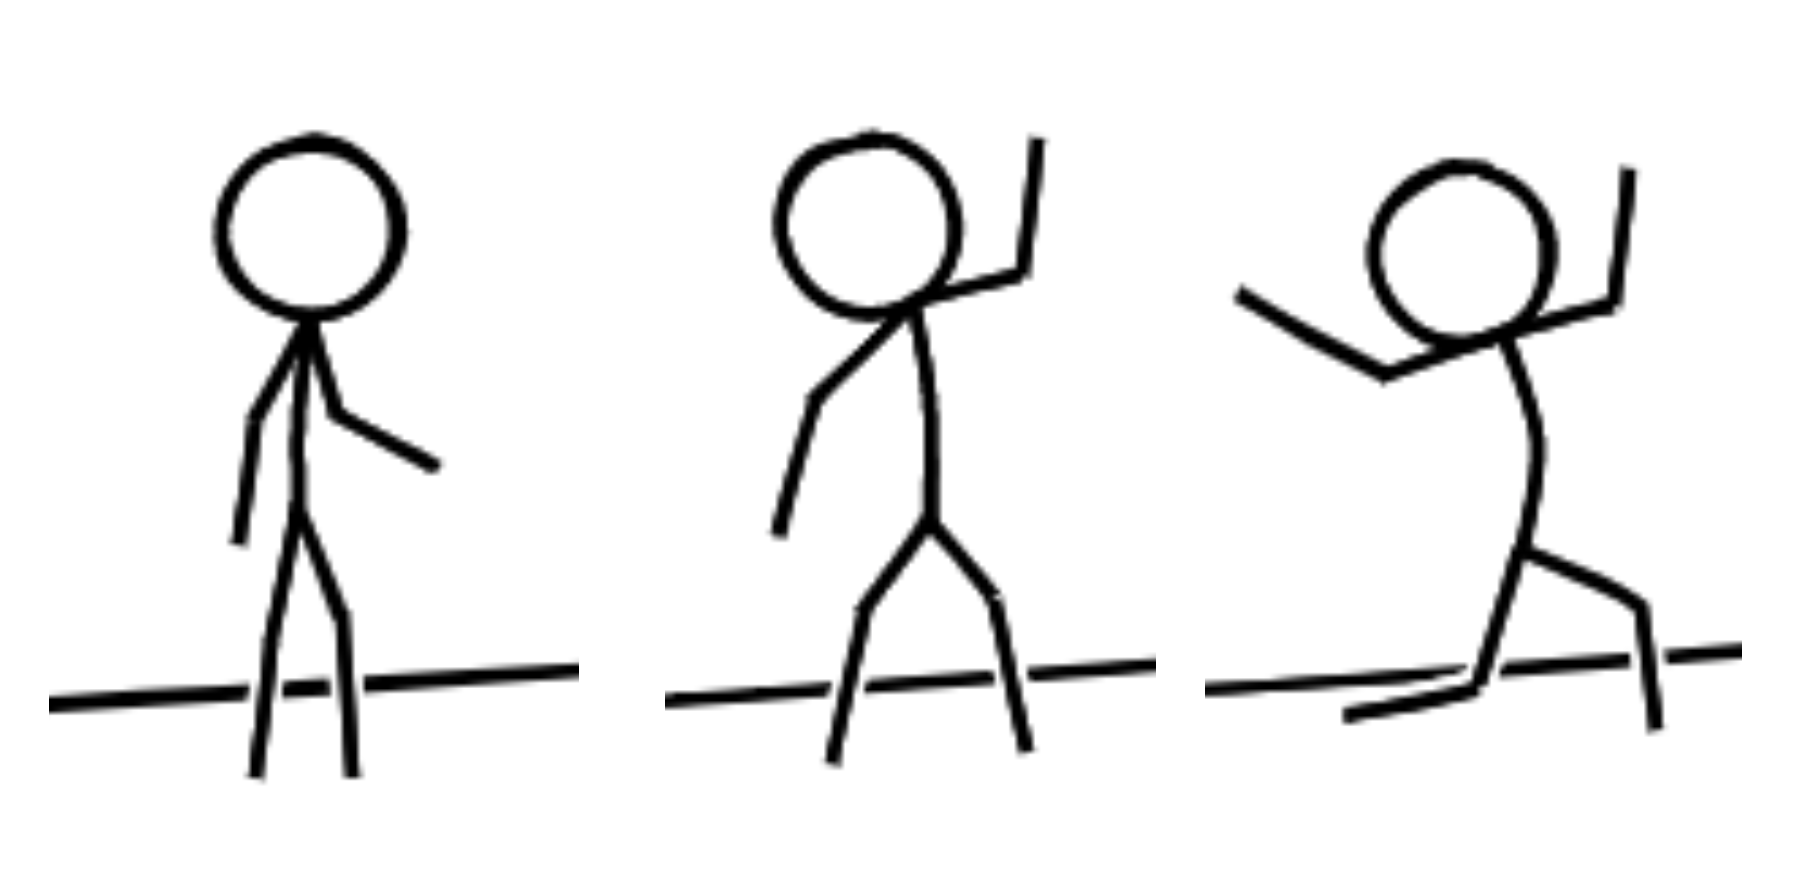
\includegraphics[width = 0.4\columnwidth]{figures/pos_figures}} &
		\subfloat[Gesture for negative framed messages ]{\label{figur:1b}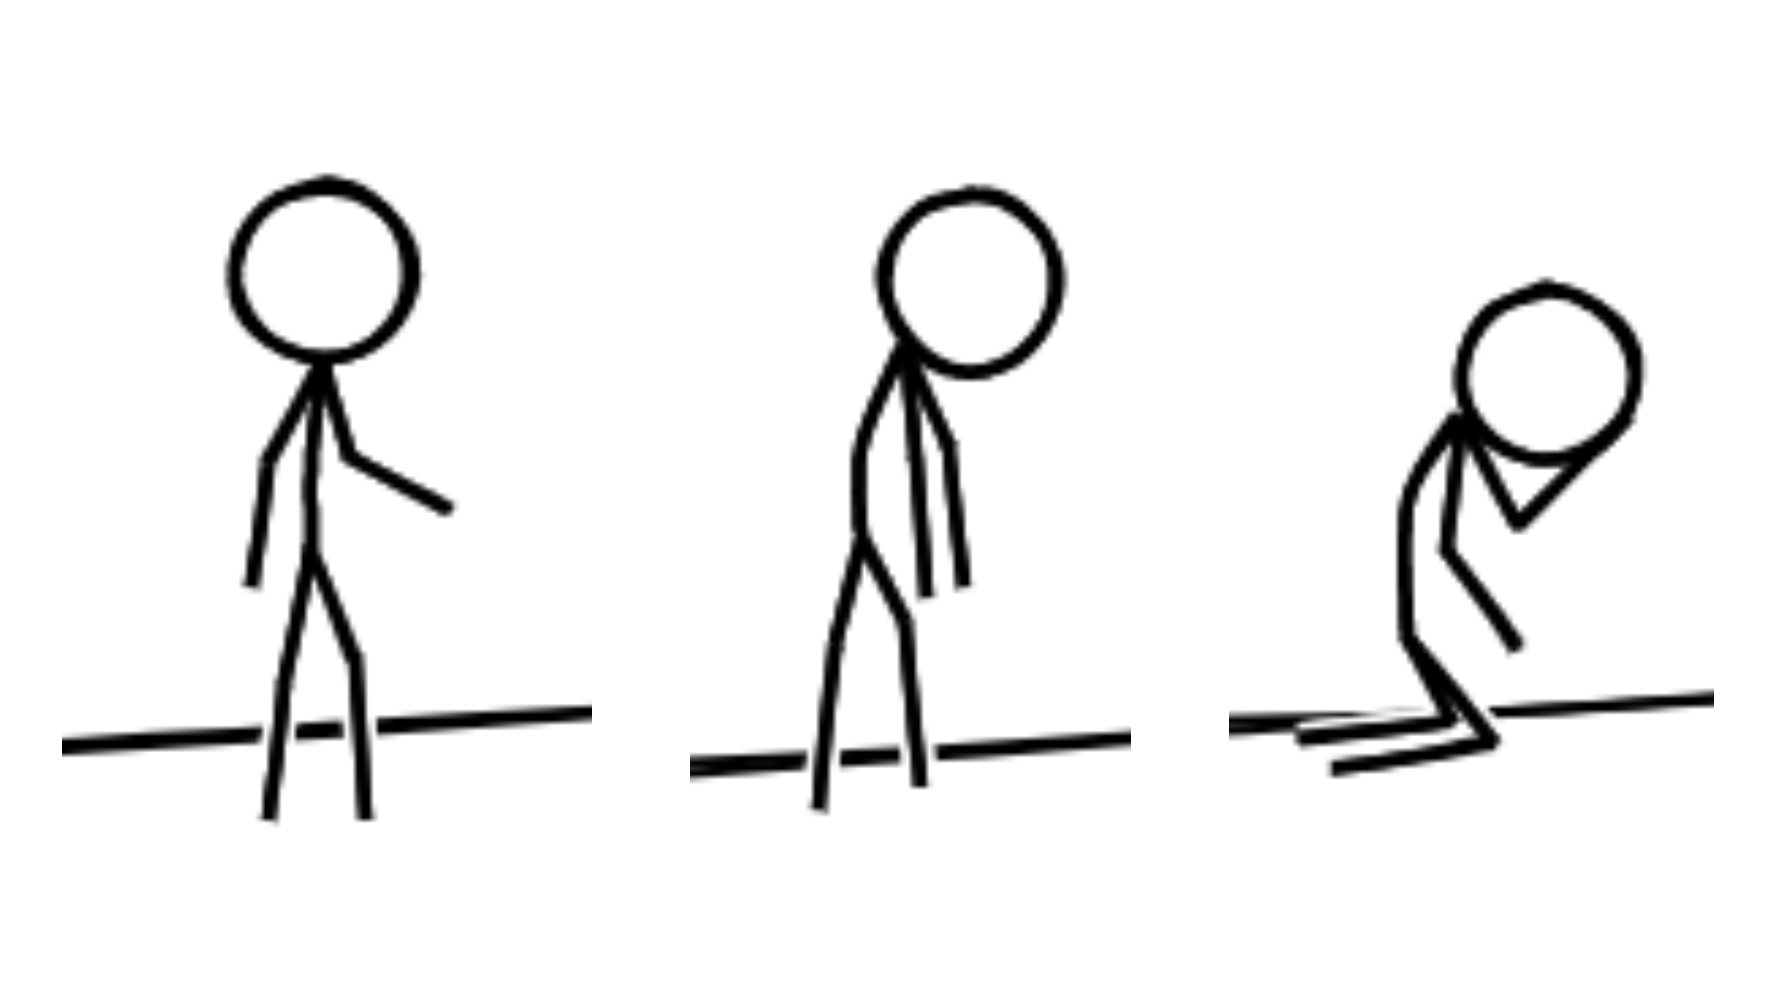
\includegraphics[width = 0.4 \columnwidth]{figures/neg_figures}}\\
	\end{tabular}
	\caption{Different character gestures to communicate various levels of emotional intensity. The left figure shows gestures used in positive framed messages from neutral to the happiest. The right figure shows gesture used in negative framed messages from neutral to the most frustrated. }
	\label{figur:figures}
\end{figure}

% \begin{figure}[t]
% 	\centering
% 	\begin{tabular}{ccc}
% 		\subfloat[Close Friends]{\label{figur:3a}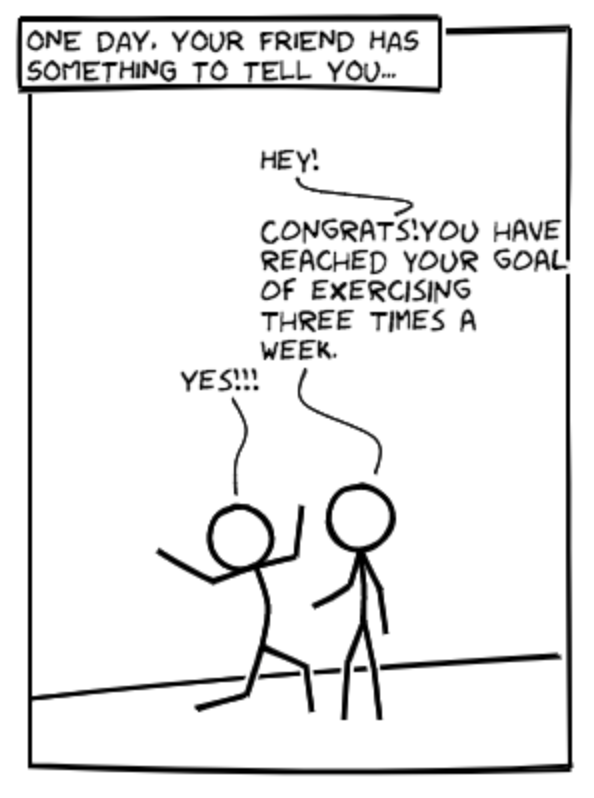
\includegraphics[width = 0.27\columnwidth]{figures/d0}} &
% 		\subfloat[Friends]{\label{figur:3b}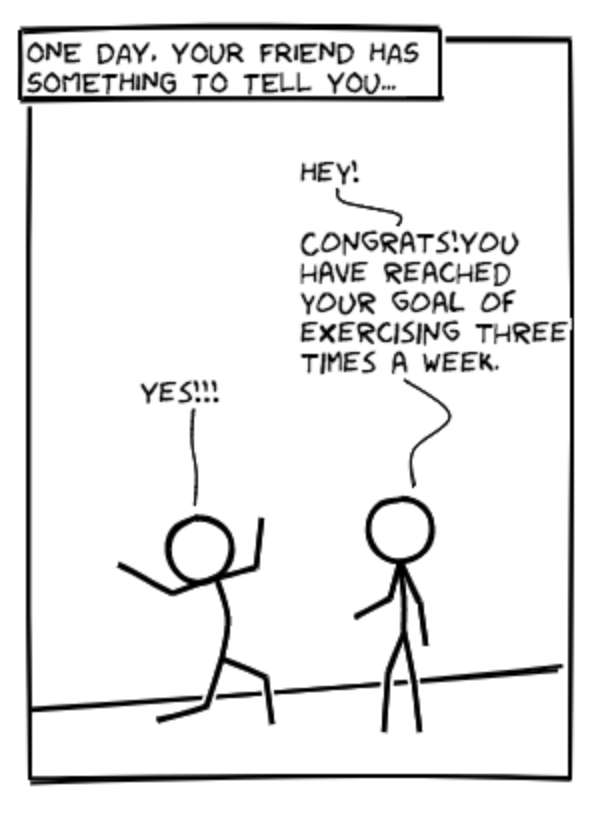
\includegraphics[width = 0.27 \columnwidth]{figures/d1}}      &
% 		\subfloat[Acquaintance]{\label{figur:3c}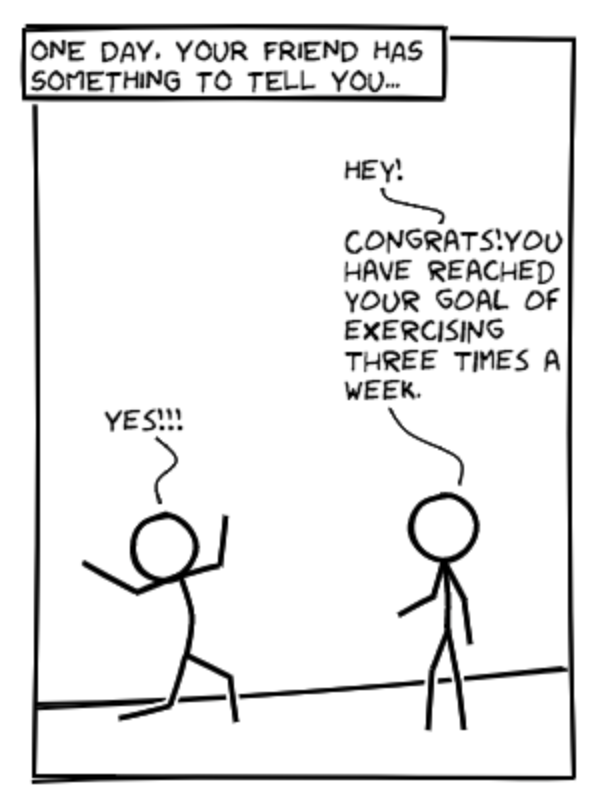
\includegraphics[width = 0.27 \columnwidth]{figures/d2}}\\
% 	\end{tabular}
% 	\caption{Different distance to communicate various levels of relationship closeness}
% 	\label{figur:distance}
% \end{figure}

To make a fair comparison between plain text representation and the comic form, the content of text bubble is the same in both conditions. We discuss generation of elements of gesture, distance between characters and shading below.

\begin{description}
	\item[Gesture]: We created the gesture library with two main categories: positive and negative corresponding to how the original message is framed, each with three levels of emotional intensity see Figure~\ref{figur:figures}.
	\item[Inter-character distance]: For the distance between two characters, we have three levels of variance from close to medium separation to large separation. The three levels of distance represents the relationship between to characters as close friends, friends, and acquaintances.
	\item[Shading]: For the background shading, we have three-levels , white, grey, and dark grey. Each color represents a level of emotional intensity correspondingly, white as ~\cite{scott1993understanding}.
\end{description}


% \begin{figure}[]
% 	\centering
% 	\begin{tabular}{ccc}
% 		\subfloat[Lowest]{\label{figur:4a}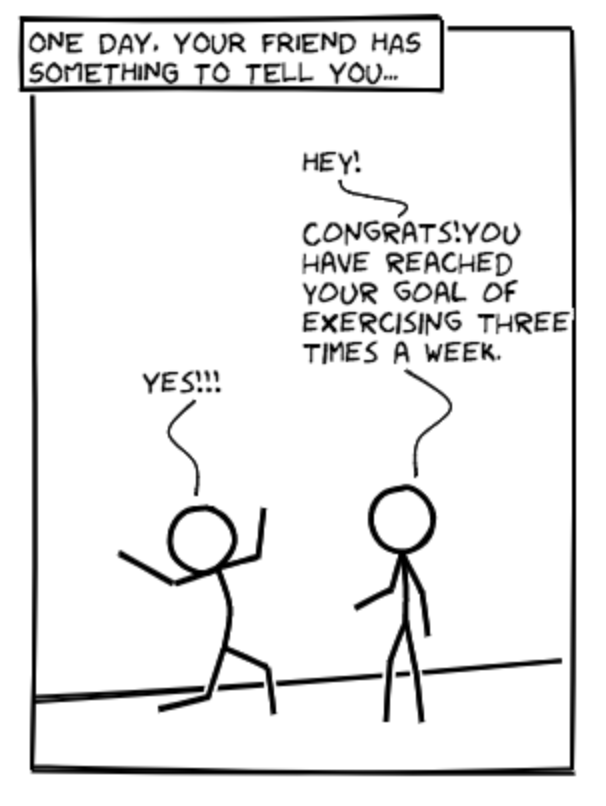
\includegraphics[width = 0.27\columnwidth]{figures/s0}}    &
% 		\subfloat[Moderate]{\label{figur:4b}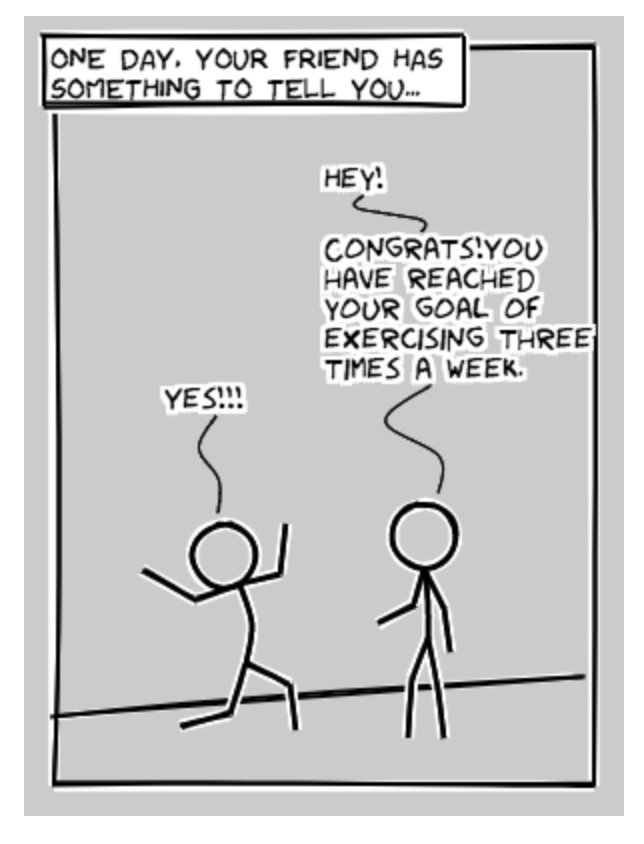
\includegraphics[width = 0.27 \columnwidth]{figures/s1}} &
% 		\subfloat[Intense]{\label{figur:4c}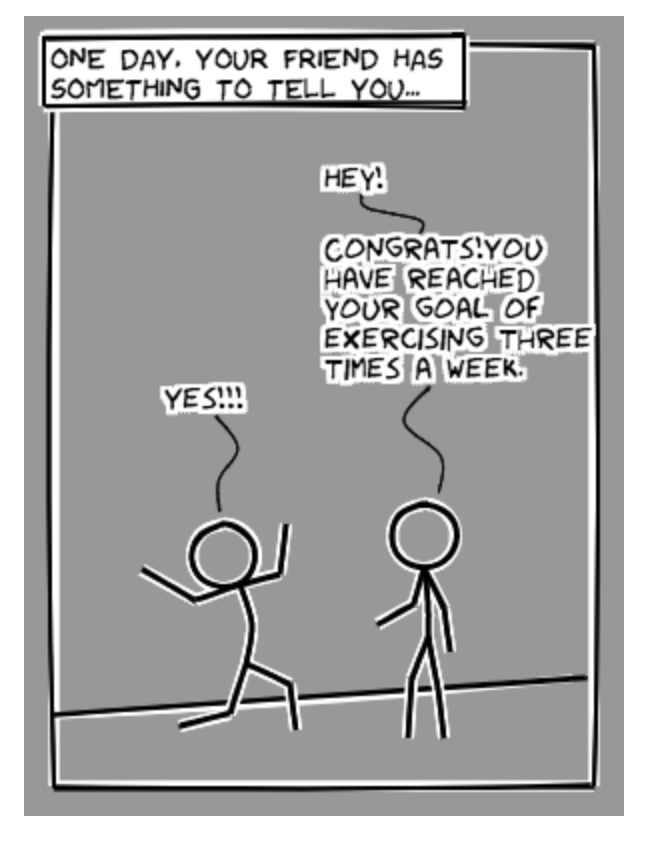
\includegraphics[width = 0.27 \columnwidth]{figures/s2}}\\
% 	\end{tabular}
% 	\caption{Different background to communicate various levels of emotional intensity}
% 	\label{figur:shading}
% \end{figure}

In total, for each message we have a total of $3 \times 3 \times 3 \times 2 =54$ variations in terms of character gesture, inter-character, background shading, and message framing. In this study, we created 270 comic form messages corresponding to 5 plain text messages.

Since the prior work~\cite{goldstein2008room,schultz2007constructive} suggests a robust effect of the social proof, instead of using it as part of an experimental condition, we will have two characters in the comic, shown as friends or the experimenter, whose inter-character distance we manipulate. Second, we will incorporate framing in the text bubbles accompanying the comic.

\subsection{Study Design}
To answer our research questions, we designed and after IRB approval, conducted a between-subject online study on Amazon Mechanical Turk.

\textit{Experiment Procedure.} Once participant consented to join our study, they were randomly assigned to two conditions 1) Positive message condition where all persuasive messages are framed in a positive way and 2) Negative condition where all persuasive messages are framed in a negative way. In both conditions, participants will see a total of five persuasive messages in both plain-text representation and comic representation shown side by side. Then, the participant rates which representation of the message is perceived as more persuasive on a 7-item Likert scale.

\textit{Display Order.} To mitigate any potential bias toward the display order of the plain-text representation and comic representation we randomize the display order. Both plain-text representation and comic-style representation have equal chance to show on the left side.

\textit{Attention Checker.} To control the data quality, we embedded two attention checkers in the study. The first one appears after the third comparison and the second one shows up after the last comparison. Both attention checkers asked subjects to choose a comic that matches a simple description, e.g. ``Which of the following comics has two characters?''

\textit{Rating Scale Design.} The 7-item Likert scale ranges from -3 (left) to 3 (right) where 0 means neutral. The direction of the scale flips corresponding to the position of the comic and plain text.
%see the right part of Figure~\ref{fig:change}.

\textit{A Pilot Study.} Before the experiment, we first conducted a pilot study with 10 participants and collect their opinions about the study process and design. Based on the feedback from our pilot test, we iterated our study design. In the final design, we fixed the order of the rating scale. However, since the order is fixed, potential demand characteristics may be introduced by the scale direction~\cite{orne1962social}. To minimize potential bias we added another layer of randomness in our final design. The direction of the scale no longer changes respect to the position of the messages within subjects, but the direction of the scale is randomly assigned between subjects. Also, we replaced the numbers on the scale by text as neutral, slightly persuasive, text/comics is more persuasive and strongly persuasive. Finally, we adjusted the size of the comic and text to make sure both of them have similar readability.
%
% The left side of Figure~\ref{fig:change} shows the final design. Another round of pilot study with another 10 participants showed the newer design successfully addressed the problems in the old design and we encountered no new problems.

% \begin{figure}
%  \centering
%  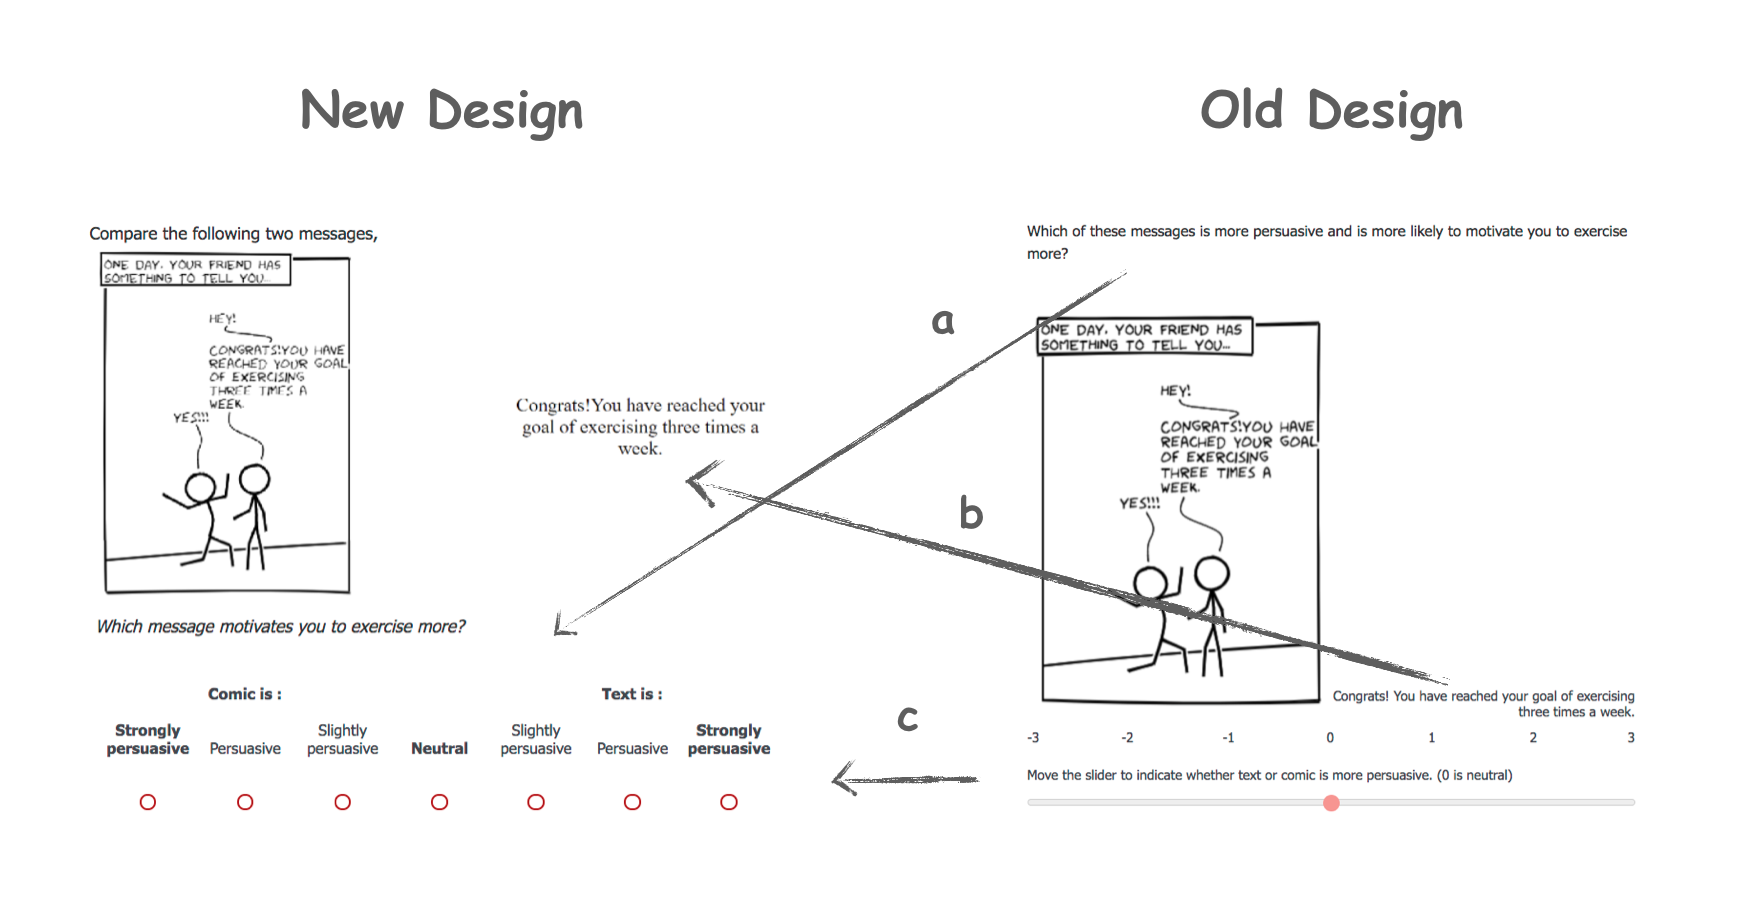
\includegraphics[width=0.95\columnwidth]{figures/change}
%  \caption{Design of the task before and after the pilot study. A. Change the position of the question to makes the question more clear. B. Adjust the position and the size of the text message to improve readability. C. Improve the rating scale to make it easy to interpreted.}
%  \label{fig:change}
% \end{figure}


\subsubsection{Participants}
We published our HITs on the Amazon Mechanical Turk titled with ``A short survey about your exercise motivation.'' The price tag for each HIT was \$8/hr, and the workers would get these rewards regardless of their performance. The threshold for participant to join our study was a 95\% Approval Rate. On the HIT page, participants would see a link to our experiment site. Workers who repeat the task will be rejected as we instructed in the task description.

\newpage
%!TEX root = cscw2019-comic.tex
\section{Study on Persuasion: Results}
\label{sec:Study on Behavior Results}

\subsection{Raw Data}
\label{sub:Study on Behavior Raw Data}
In total we have 307 participants joined our study, 101 participants received the message in the text form, 102 participants received the same message in the comic form, and 104 participants received the comic message with social-proof. We ran an outlier analysis on participants' completion time and removed 30 participants from our dataset. The following analysis is based on a dataset with 277 participants, 91 of them is in pure-text condition, 97 of them is in comic condition, and 92 of them is in comic-social-proof condition. Of those 277 participants, 150 were self-identified as male, and 126 were self-identified as female, 1 participant chose not to disclose. 197 participants earned at least college degree.

\begin{figure*}[htb]
	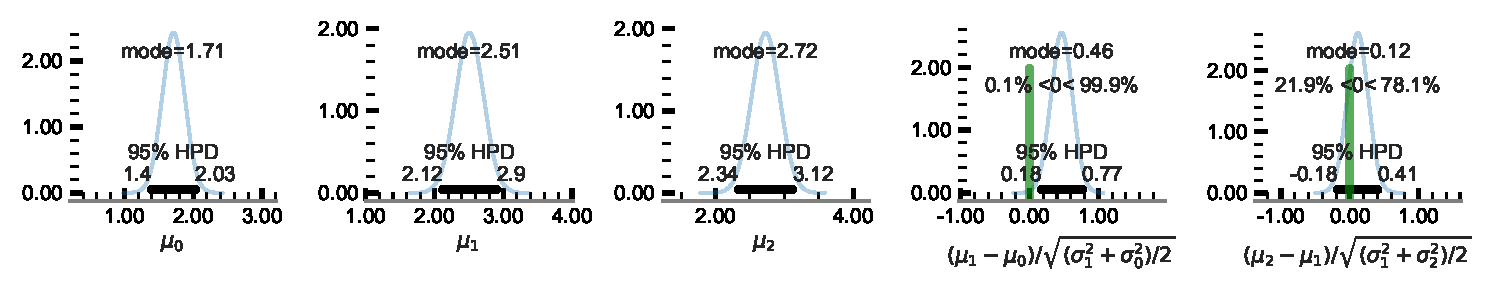
\includegraphics[width=1\textwidth]{./hari-code/new_exp_text_v_comic_v_social.pdf}
    \caption{The posterior distribution of the amount of money participants decide to donate to the charity in each of the three conditions: text only ($\mu_0$); comic ($\mu_1$); comic with social norm ($\mu_2$). The right two panels are respectively: posterior distribution of the effect size contrasting the comic condition ($\mu_1$) and text ($\mu_0$); the effect size contrasting comic with social norm ($\mu_2$) with the plain comic ($\mu_1$). First notice that $\mu_2 > \mu_1 > \mu_0$. Furthermore, the modal effect size of comparing the comic panel against text is 0.48, a medium effect and the HPD interval $[0.17, 0.77]$ reliably excludes a ROPE of $[0 \pm 0.1]$, indicating that the effect is meaningful. The effect of introducing the social norm into the comic has a minor effect (mode=0.12) when contrasted against the plan comic, and the HPD interval $[-0.17, 0.41]$ includes a ROPE of $[0 \pm 0.1]$, indicating that the outcome is not convincing.}
	\label{fig:main-experiment2-effect}
\end{figure*}

\subsection{Analysis}
\label{sub:Study on Behavior Analysis}

Now, we discuss our Bayesian formulation. There is one outcome variable $y_{i \mid j}$, the amount of donation to the charity by each participant $i$, under experimental condition $j$: text, comic, and comic with social norm. Our Bayesian model:

\begin{align}
    y_{i \mid j} \sim &  \mathrm{StudentT}(\nu, \mu_j, \sigma_j), \\
    \nu \sim & \exp(\lambda), \\
    \mu_j \sim & N(a,b), \\
    \sigma_j \sim & U(L,H).
\end{align}

We use a $\mathrm{StudentT}$ distribution with $\nu$ degrees of freedom to model the random variable; notice that this is a \textit{drawing distribution}, not the $t$-test. The $\mathrm{StudentT}$ allows us to model a non-Normal outcome with a heavy tail; assuming $y_{i \mid j}$ to be Normally distributed is equivalent to setting $\nu=\infty$. The degrees of freedom $\nu$ is drawn from an exponential distribution; the mode $\mu_j$ corresponding to each experimental group is drawn from a Normal distribution; the ``width'' $\sigma_j$ of the $t$-distribution corresponding to group $j$ is drawn from an uniform distribution. The hyper-priors for variables $\nu$, $\mu_j$ and $\sigma_j$ are set to be generous to allow for wide variation in these values. For example, we set $\lambda=\sfrac{1}/{29}$, since $\nu \geq 30$ is a rule of thumb for presence of Normality.

The result ~\Cref{fig:main-experiment2-effect} shows the modal effect size between abstract-comic v. pure-text = 0.48; There is no overlap of the 95\% high probability density (HPD) interval with the ROPE of [-0.1, 0.1]. Thus the effect is of medium size and meaningful; the effect size between abstract-comic and social-proof-comic is 0.12; but since the distribution includes a ROPE of $[-0.1 \pm 0.1]$, the effect is not convincing.

In this section, we presented a Bayesian model to analyze the overall effect of using a abstract-comic to persuade people making charitable donation decisions, and understand the effect of adapting persuasive techniques in the abstract comic form. The results show that the use of abstract-comic produces a significant effect in persuading participants to donate. Although abstract-comic with social proof can produce larger effect, the contrast between abstract-comic and abstract-comic with social proof is not significant. Next we discuss the findings, limitations and design implications.

\newpage
\section{Discussion}
% \newpage
% \section{Acknowledgments}
% \section{References}





% Use a numbered list of references at the end of the article, ordered
% alphabetically by first author, and referenced by numbers in
% brackets~\cite{ethics, Klemmer:2002:WSC:503376.503378,
%   Mather:2000:MUT, Zellweger:2001:FAO:504216.504224}. For papers from
% conference proceedings, include the title of the paper and an
% abbreviated name of the conference (e.g., for Interact 2003
% proceedings, use \textit{Proc. Interact 2003}). Do not include the
% location of the conference or the exact date; do include the page
% numbers if available. See the examples of citations at the end of this
% document. Within this template file, use the \texttt{References} style
% for the text of your citation.

% Your references should be published materials accessible to the
% public.  Internal technical reports may be cited only if they are
% easily accessible (i.e., you provide the address for obtaining the
% report within your citation) and may be obtained by any reader for a
% nominal fee.  Proprietary information may not be cited. Private
% communications should be acknowledged in the main text, not referenced
% (e.g., ``[Robertson, personal communication]'').


\balance{}


% REFERENCES FORMAT
% References must be the same font size as other body text.
\bibliographystyle{SIGCHI-Reference-Format}
\bibliography{sample}

\end{document}

%%% Local Variables:
%%% mode: latex
%%% TeX-master: t
%%% End:
